
\documentclass[a4paper,11pt]{article}%,twocolumn
%% packages

\usepackage{blindtext} % needed for creating dummy text passages
%\usepackage{ngerman} % needed for German default language
\usepackage{amsmath} % needed for command eqref
\usepackage{amssymb} % needed for math fonts
\usepackage[colorlinks=true,breaklinks]{hyperref} % needed for creating hyperlinks in the document, the option colorlinks=true gets rid of the awful boxes, breaklinks breaks lonkg links (list of figures), and ngerman sets everything for german as default hyperlinks language
\usepackage[hyphenbreaks]{breakurl} % ben�tigt f�r das Brechen von URLs in Literaturreferenzen, hyphenbreaks auch bei links, die �ber eine Seite gehen (mit hyphenation).
\usepackage{xcolor}
\definecolor{c1}{rgb}{0,0,1} % blue
\definecolor{c2}{rgb}{0,0.3,0.9} % light blue
\definecolor{c3}{rgb}{0.3,0,0.9} % red blue
\hypersetup{
    linkcolor={c1}, % internal links
    citecolor={c2}, % citations
    urlcolor={c3} % external links/urls
}
%\usepackage{cite} % needed for cite
\usepackage[square,authoryear]{natbib} % needed for cite and abbrvnat bibliography style
\usepackage[nottoc]{tocbibind} % needed for displaying bibliography and other in the table of contents
\usepackage{graphicx} % needed for \includegraphics 
\usepackage{longtable} % needed for long tables over pages
\usepackage{bigstrut} % needed for the command \bigstrut
\usepackage{enumerate} % needed for some options in enumerate
%\usepackage{todonotes} % needed for todos
\usepackage{makeidx} % needed for creating an index
\makeindex
\usepackage{gensymb}
\usepackage{url}
\usepackage{psfrag}
\usepackage{multirow}
\usepackage{subfigure}
%% page settings

\usepackage[top=20mm, bottom=20mm,left=15mm,right=15mm]{geometry} % needed for page border settings
\parindent=0mm % for space of first line of new text block
\sloppy % for writing with hyphenless justification (tries to)
\hyphenation{} % use hyphenation of tolerance parametershttp://www.jr-x.de/publikationen/latex/tipps/zeilenumbruch.html
\hyphenpenalty=10000
\exhyphenpenalty=10000
\usepackage{fancyhdr} % needed for head and foot options
%% my macros

%% Text fomats
\newcommand{\tbi}[1]{\textbf{\textit{#1}}}

%% Math fonts
\newcommand{\bbA}{\mathbb{A}}
\newcommand{\bbB}{\mathbb{B}}
\newcommand{\bbC}{\mathbb{C}}
\newcommand{\bbD}{\mathbb{D}}
\newcommand{\bbE}{\mathbb{E}}
\newcommand{\bbF}{\mathbb{F}}
\newcommand{\bbG}{\mathbb{G}}
\newcommand{\bbH}{\mathbb{H}}
\newcommand{\bbI}{\mathbb{I}}
\newcommand{\bbJ}{\mathbb{J}}
\newcommand{\bbK}{\mathbb{K}}
\newcommand{\bbL}{\mathbb{L}}
\newcommand{\bbM}{\mathbb{M}}
\newcommand{\bbN}{\mathbb{N}}
\newcommand{\bbO}{\mathbb{O}}
\newcommand{\bbP}{\mathbb{P}}
\newcommand{\bbQ}{\mathbb{Q}}
\newcommand{\bbR}{\mathbb{R}}
\newcommand{\bbS}{\mathbb{S}}
\newcommand{\bbT}{\mathbb{T}}
\newcommand{\bbU}{\mathbb{U}}
\newcommand{\bbV}{\mathbb{V}}
\newcommand{\bbW}{\mathbb{W}}
\newcommand{\bbX}{\mathbb{X}}
\newcommand{\bbY}{\mathbb{Y}}
\newcommand{\bbZ}{\mathbb{Z}}
\usepackage[ framed, numbered]{matlab-prettifier}%framed,%
\usepackage{listings}
\usepackage{physics}
\usepackage{pdfpages}
\usepackage[toc,page]{appendix}
\usepackage{float}
\usepackage{pifont}


\begin{document}
\begin{titlepage}
\center % Center everything on the page

%-------------------------------------------------------------------------------------
%	HEADING SECTIONS
%------------------------------------------------------------------------------------
\textbf{\large Department of Electrical and Computer Engineering}\\[0.5cm]
\textbf{\Large University of Colorado at Boulder}\\[1cm]
\textbf{\large ECEN5730 - Practical PCB design}\\[2cm]

\includegraphics[width=0.3\textwidth]{figures/cu}\\[2cm] 

	
%-------------------------------------------------------------------------------------
%	TITLE SECTION
%------------------------------------------------------------------------------------

\textbf{\Huge Board Good Layout/Bad Layout }\\[0.2cm]

\textbf{\Large Report}\\[2cm]
\vspace{1.5cm}
\begin{figure}[H]
	\centering
	
\includegraphics[scale=0.2]{figures/qr_download.png}
	\label{555_schematic}
\end{figure}\vspace{1.5cm}


%----------------------------------------------------------------------------------------
%	MEMBERS SECTION
%----------------------------------------------------------------------------------------


\vfill

\textbf{\large Submitted by}

{\large Parth Thakkar}\\[0.5cm]




%----------------------------------------------------------------------------------------
%	DATE SECTION
%----------------------------------------------------------------------------------------

\textbf{\large Submitted on}\\
\textbf{\Large \today} % Date, change the \today to a set date if you want to be precise

%----------------------------------------------------------------------------------------

\vfill % Fill the rest of the page with whitespace

\end{titlepage}

\pagebreak

\tableofcontents
\listoffigures
\listoftables
\vfill
\begin{center}
	\textbf{\textit{*PDF is clickable}}
\end{center}

\pagebreak

\section{Introduction}


1. This board design brings together and demonstrates how to implement interconnect
design features to reduce the two important switching noise sources: on the PDN and
between signal-return paths.

\textbf{Measurements to be Conducted:}

\begin{enumerate}
	\item \textbf{Voltage Measurement:} Check the voltage at the output pin of the 555 timer with 5V and 3.3V power supply and check switching noise in both cases
	\item \textbf{Oscilloscope Analysis:} Use an oscilloscope equipped with a 10x probe to observe the rise and fall times of the 555 timer's output signal. Enable good layout and measure quiet high and quite low in the good layout with rising and falling edge, measure peak to peak noise
	\item \textbf{Noise Measurement:} Examine the switching noise in bad layout by turing on bad layout with switch and measure quite high and quite low in bad layout with respect to rising and falling edge.
	\item measure Voltage drop across good layout's output and measure Thevenin resistance of hex inverter
\end{enumerate}

For the construction, 1206 size surface-mount device (SMD) components were chosen and soldered onto a printed circuit board (PCB). This choice of components and the assembly process highlight the practical aspects of PCB design flow, from selecting appropriate parts to the actual soldering and testing of the finished board.

\section{Project Plan}
\begin{enumerate}
	\item Integrate an external power source connector for a 5V AC to DC adapter to supply power to the circuit board.
	\item Implement a voltage converter to step down from 5V to 3.3V.
	\item Incorporate a high-speed 555 Timer IC.
	\item Design the timer circuit to achieve approximately 500 Hz frequency with a 66\% duty cycle.
	\item Configure the circuit to activate four inputs of a hex inverter, illustrating both effective and poor circuit layouts.
	\item Employ red LEDs and 50 ohm resistors as loads for three of the switch outputs from each hex inverter.
	\item Calculate the current consumption by the inverter for the combined load of the LED and the 50 ohm resistor.
	\item Determine the Thevenin equivalent resistance at the output terminal of one of the I/O pins.
	\item Design one side of the printed circuit board (PCB) using optimal layout practices and the opposite side with suboptimal layout techniques. In the less effective layout, position the decoupling capacitors significantly away from the Vcc pin.
	\item  Ensure consistent component placement and routing across both sections of the PCB, with the exception of the decoupling capacitor's positioning.
	\item  Establish test points for the following signals:
	\begin{itemize}
		\item The oscilloscope trigger output
		\item Voltage across a 50 ohm resistor
		\item Voltage at the output of an inverter driving the LED and resistor load
		\item The high signal level in a quiescent state
		\item The low signal level in a quiescent state
		\item The 555 timer output signal
		\item The 3.3V power rail on the PCB
		\item The 5V power rail on the PCB
	\end{itemize}
	
	\item Add a decoupling capacitor for the 555 timer IC to mitigate switching noise.
	\item Implement a copper pour for the ground plane to enhance circuit stability.
	\item Incorporate indicator lights, testing points, and isolation switches for comprehensive functionality and diagnostic capabilities.
\end{enumerate}



\section{Risk Management}
\begin{enumerate}
	\item Test points will be strategically placed and clearly labeled for easy identification.
	\item Isolation switches will be installed at each stage to facilitate troubleshooting and debugging.
	\item The 555-timer will be chosen based on the required output current to ensure proper operation.
	\item Signal lines will have a width of 6 mils to maintain signal integrity.
	\item Power lines will be designed with a width of 20 mils to distinguish them easily and support adequate current flow.
	\item Good layout will have all the good prectices like keeping traces short, keeping decoupling cap close to IC, having ground plane.
	\item Bad layout will have all the bad prectices like keeping decoupling capacitor as far as possible, not having ground plane.
	\item The output from Altium Designer will be checked for feasibility, with Gerber files generated and tested for manufacturing.
	\item The schematic will be compared with the breadboard implementation of 555 and hex board to ensure the design works as intended in a practical setting.
	
\end{enumerate}

\section{Block Diagram, Schematic and Layout}

\subsection{Block Diagram Description}
\subsubsection{555}
The block diagram for the 555 timer PCB project is divided into three main sections:

\begin{enumerate}
	\item Power Supply(LDO): This section includes the external 5V AC to DC charger input, and convert it in to 3.3v ensuring the board receives a stable power supply. It is isolated from the rest of the circuit to prevent noise interference.
	\item 555 Timer Circuit: The core of the project, where the 555 timer IC operates in an astable mode to generate a variable frequency output. This section is designed to allow adjustments in the duty cycle through a potentiometer and is isolated for easy modification or debugging.
	\item Output Unit: Includes the output stage where the signal from the 555 timer is utilized. This could involve LEDs, a speaker, or other components to demonstrate the output signal's behavior. Isolation switches are also present here to detach the unit when necessary.
\end{enumerate}

\begin{figure}[H]
	\centering
	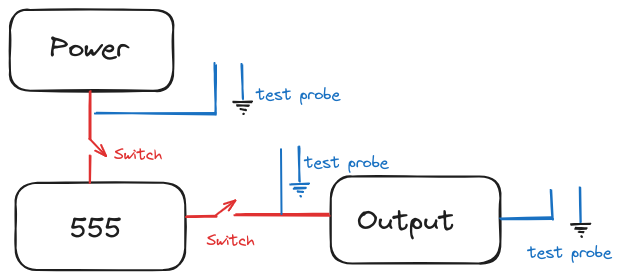
\includegraphics[scale=0.4]{figures/ne555_blockdiagram}
	\caption{Block diagram of ne555}
\end{figure}
\subsubsection{Hex board}
\begin{enumerate}
	\item Hex Inverter Gates (1 to 6): These are logic gates that invert the input signal. Gate 1 is directly connected to a scope trigger to capture the waveform for analysis. Gates 2, 3, and 4 drive LEDs through 50 $\ohm$ resistors, which likely serve as both current-limiting resistors and part of the load to assess the switching characteristics and noise levels of the inverter outputs.
	\item LEDs (9 to 11): Light-emitting diodes connected to represent the load on the outputs of the hex inverter and to visualize the switching activity.
	\item Resistors (50 $\ohm$): Connected in series with the LEDs to limit the current through them and to serve as a load for noise measurement.
	\item Test Points: The diagram includes various test points:
	\begin{itemize}
		\item To Scope Trigger: Allows for synchronization of the oscilloscope with the signal for accurate measurement.
		\item Quiet LOW (5): A test point to measure the low voltage level of the signal 
		\item Quiet HIGH (6): Similar to the Quiet LOW, this test point is to measure the high voltage level
	\end{itemize}
	
	
	\begin{figure}[H]
		\centering
		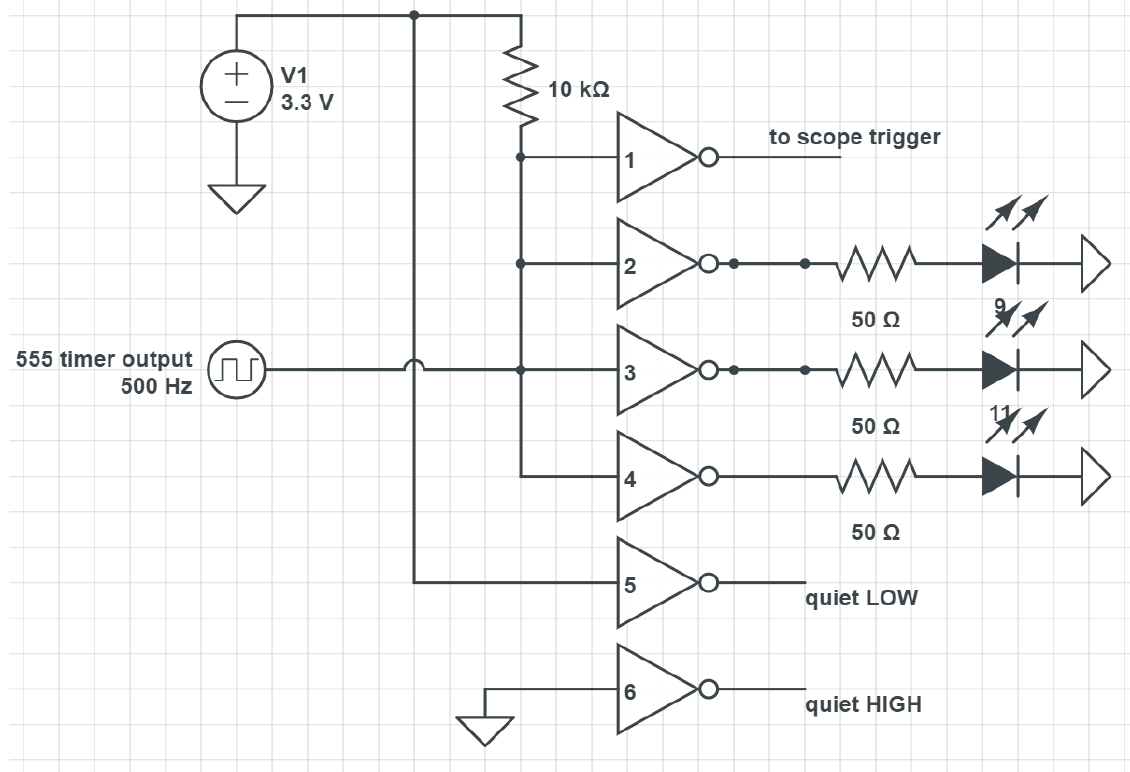
\includegraphics[scale=0.4]{figures/signal_noise.png}
		\caption{Block diagram of Hex board}
	\end{figure}
	

\end{enumerate}

The layout includes a good and bad design for comparison. In the bad design, decoupling capacitors are expected to be placed farther from the Vcc pin of the inverters, which could potentially increase the noise due to the longer traces acting as antennas or due to the inductance of the longer traces. The good layout would place the decoupling capacitors close to the Vcc pin to minimize noise.\\\\

The test points at the Quiet LOW and Quiet HIGH are critical for measuring the noise floor of the system without the impact of the switching signal.

\subsection{Component listings}
\begin{table}[H]
	\centering 
	\begin{tabular}{l c  c }
		\hline
		\textbf{Component Name}&\textbf{Usecase}&\textbf{Value}\\\hline
		&&\\

3 x Capacitor&Decoupling cap&22$\mu$F\\
2 x Capacitor&Filter Capacitor&10$\mu$F\\
2 x Capacitor&Discharging Capacitor&1$\mu$F\\
2 x 2 pin Switches&Switch for isolation&\\
1 x 3 pin Switches&Switch for selection&\\
2 x Resistor&Discharging rate Resistor&1k$\ohm$\\
1 x Resistor&Current Limiting resistor&50$\ohm$\\
1 x Resistor&Current Limiting resistor&1k$\ohm$\\
1x NE555&Timer IC&\\
1x AMS1117&LDO&\\
2x Smitt Trigger Interverter&Hex IC&\\
8 x LEDs&For output&\\
1 x connector&For power supply&\\
\hline\hline
	\end{tabular}
	\caption{Component list}
	\label{filterspecs}
\end{table}



\subsection{Schematic Overview}


\begin{figure}[H]
	\centering
	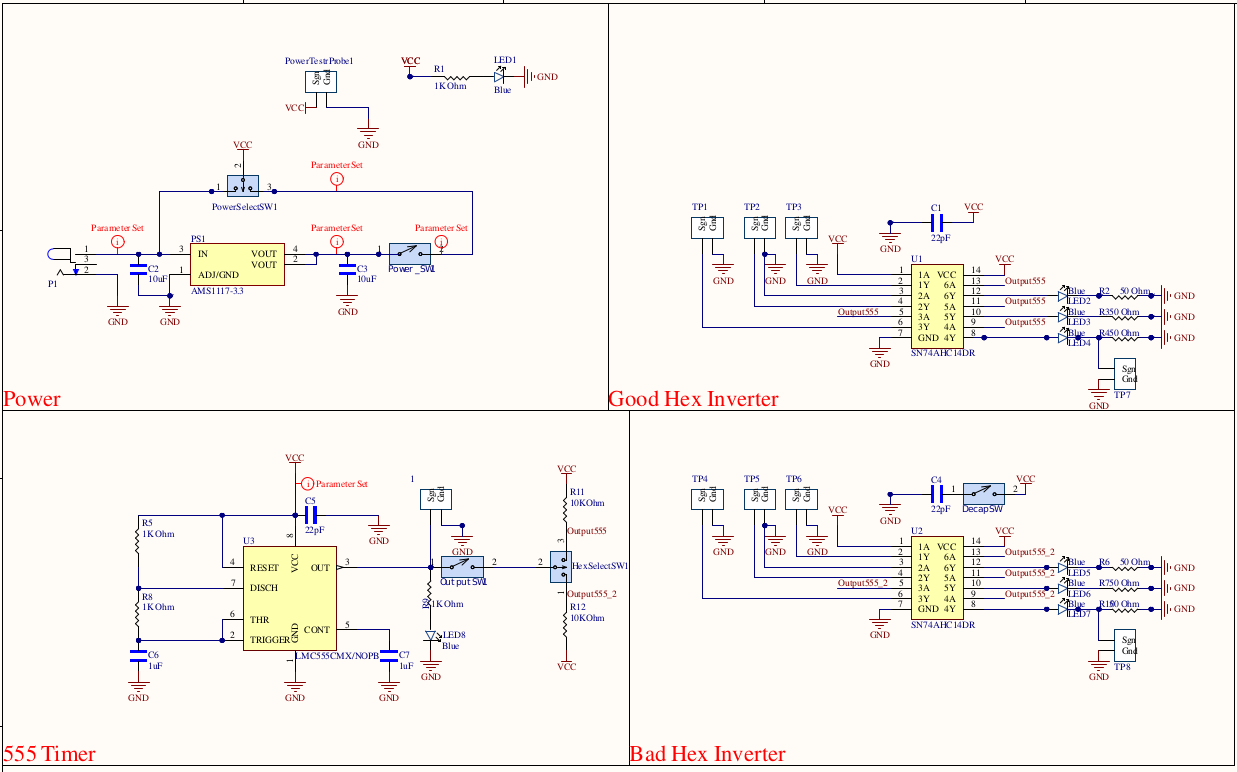
\includegraphics[scale=0.4]{figures/schematic.png}
	\caption{Schematic}
\end{figure}

\begin{enumerate}
	\item Power Section: This section converts an external 5V supply to a 3.3V output using a voltage regulator (AMS1117-3.3). Decoupling capacitors (10 µF) are placed at the input and output of the voltage regulator to stabilize the voltage and reduce noise. There's also a test point (PowerTestProbe1) and an LED (LED1) with a current-limiting resistor (R1) to indicate power status.
	\item 555 Timer Section: The 555 timer IC (U3) is configured with resistors (R5 and R6), capacitors (C5 and C7), and a diode (D1) to produce a 500 Hz square wave output. This section includes a switch (OutputSW) to enable or disable the output, an LED (LED8) to visualize the output signal, and a couple of test points (TP4, TP5, and TP6) to measure the timer's output and supply voltages.
	\item Good Hex Inverter Section: Here, a hex inverter IC (U1) with good layout practices has its VCC pin closely decoupled with a capacitor (C1). The inverter's outputs drive LEDs (Output555\_1, Output555\_2, Output555\_3) through current-limiting resistors (R2, R3, and R4). The test points (TP1, TP2, and TP3) facilitate measurements of the output signals and supply voltage.
	\item Bad Hex Inverter Section: This section uses the same type of hex inverter IC (U2) but with bad layout practices, where the decoupling capacitor (C4) is not placed close to the VCC pin, potentially leading to more noise in the signals. This section's outputs also drive LEDs (Output555\_5, Output555\_6, Output555\_7) through resistors (R9, R10, and R11). Test points (TP7, TP8, and TP9) are provided for the same purpose as in the good layout section.
	
\end{enumerate}
The primary differences between the "Good Hex Inverter" and "Bad Hex Inverter" sections are the placement of the decoupling capacitors and potentially the trace routing (not visible in the schematic). Decoupling capacitors are important for IC and for filtering out high-frequency noise. Their placement in proximity to the VCC pin is important in minimizing the loop area.



\subsection{Layout Considerations}
For the PCB layout, several factors are critical:

\begin{enumerate}
	\item \textbf{Test Probes:} Designated points for measuring power rail voltage, the output from the 555 timer, and the voltage across a 1k resistor. Each test point is accessible via individual switches for isolation.
	\item \textbf{Decoupling Capacitor:} Positioned as close to the 555 timer IC as possible to minimize switching noise and stabilize the power supply to the IC.
	\item \textbf{Ground Pour:} Implementing a ground pour around signal and power traces to enhance signal integrity and provide a better return path for signals, reducing interference and improving circuit performance.
\end{enumerate}


\pagebreak
\section{Manufacturing and Assembly}

Breadboard Implementation:


\begin{figure}[H]
	\centering
	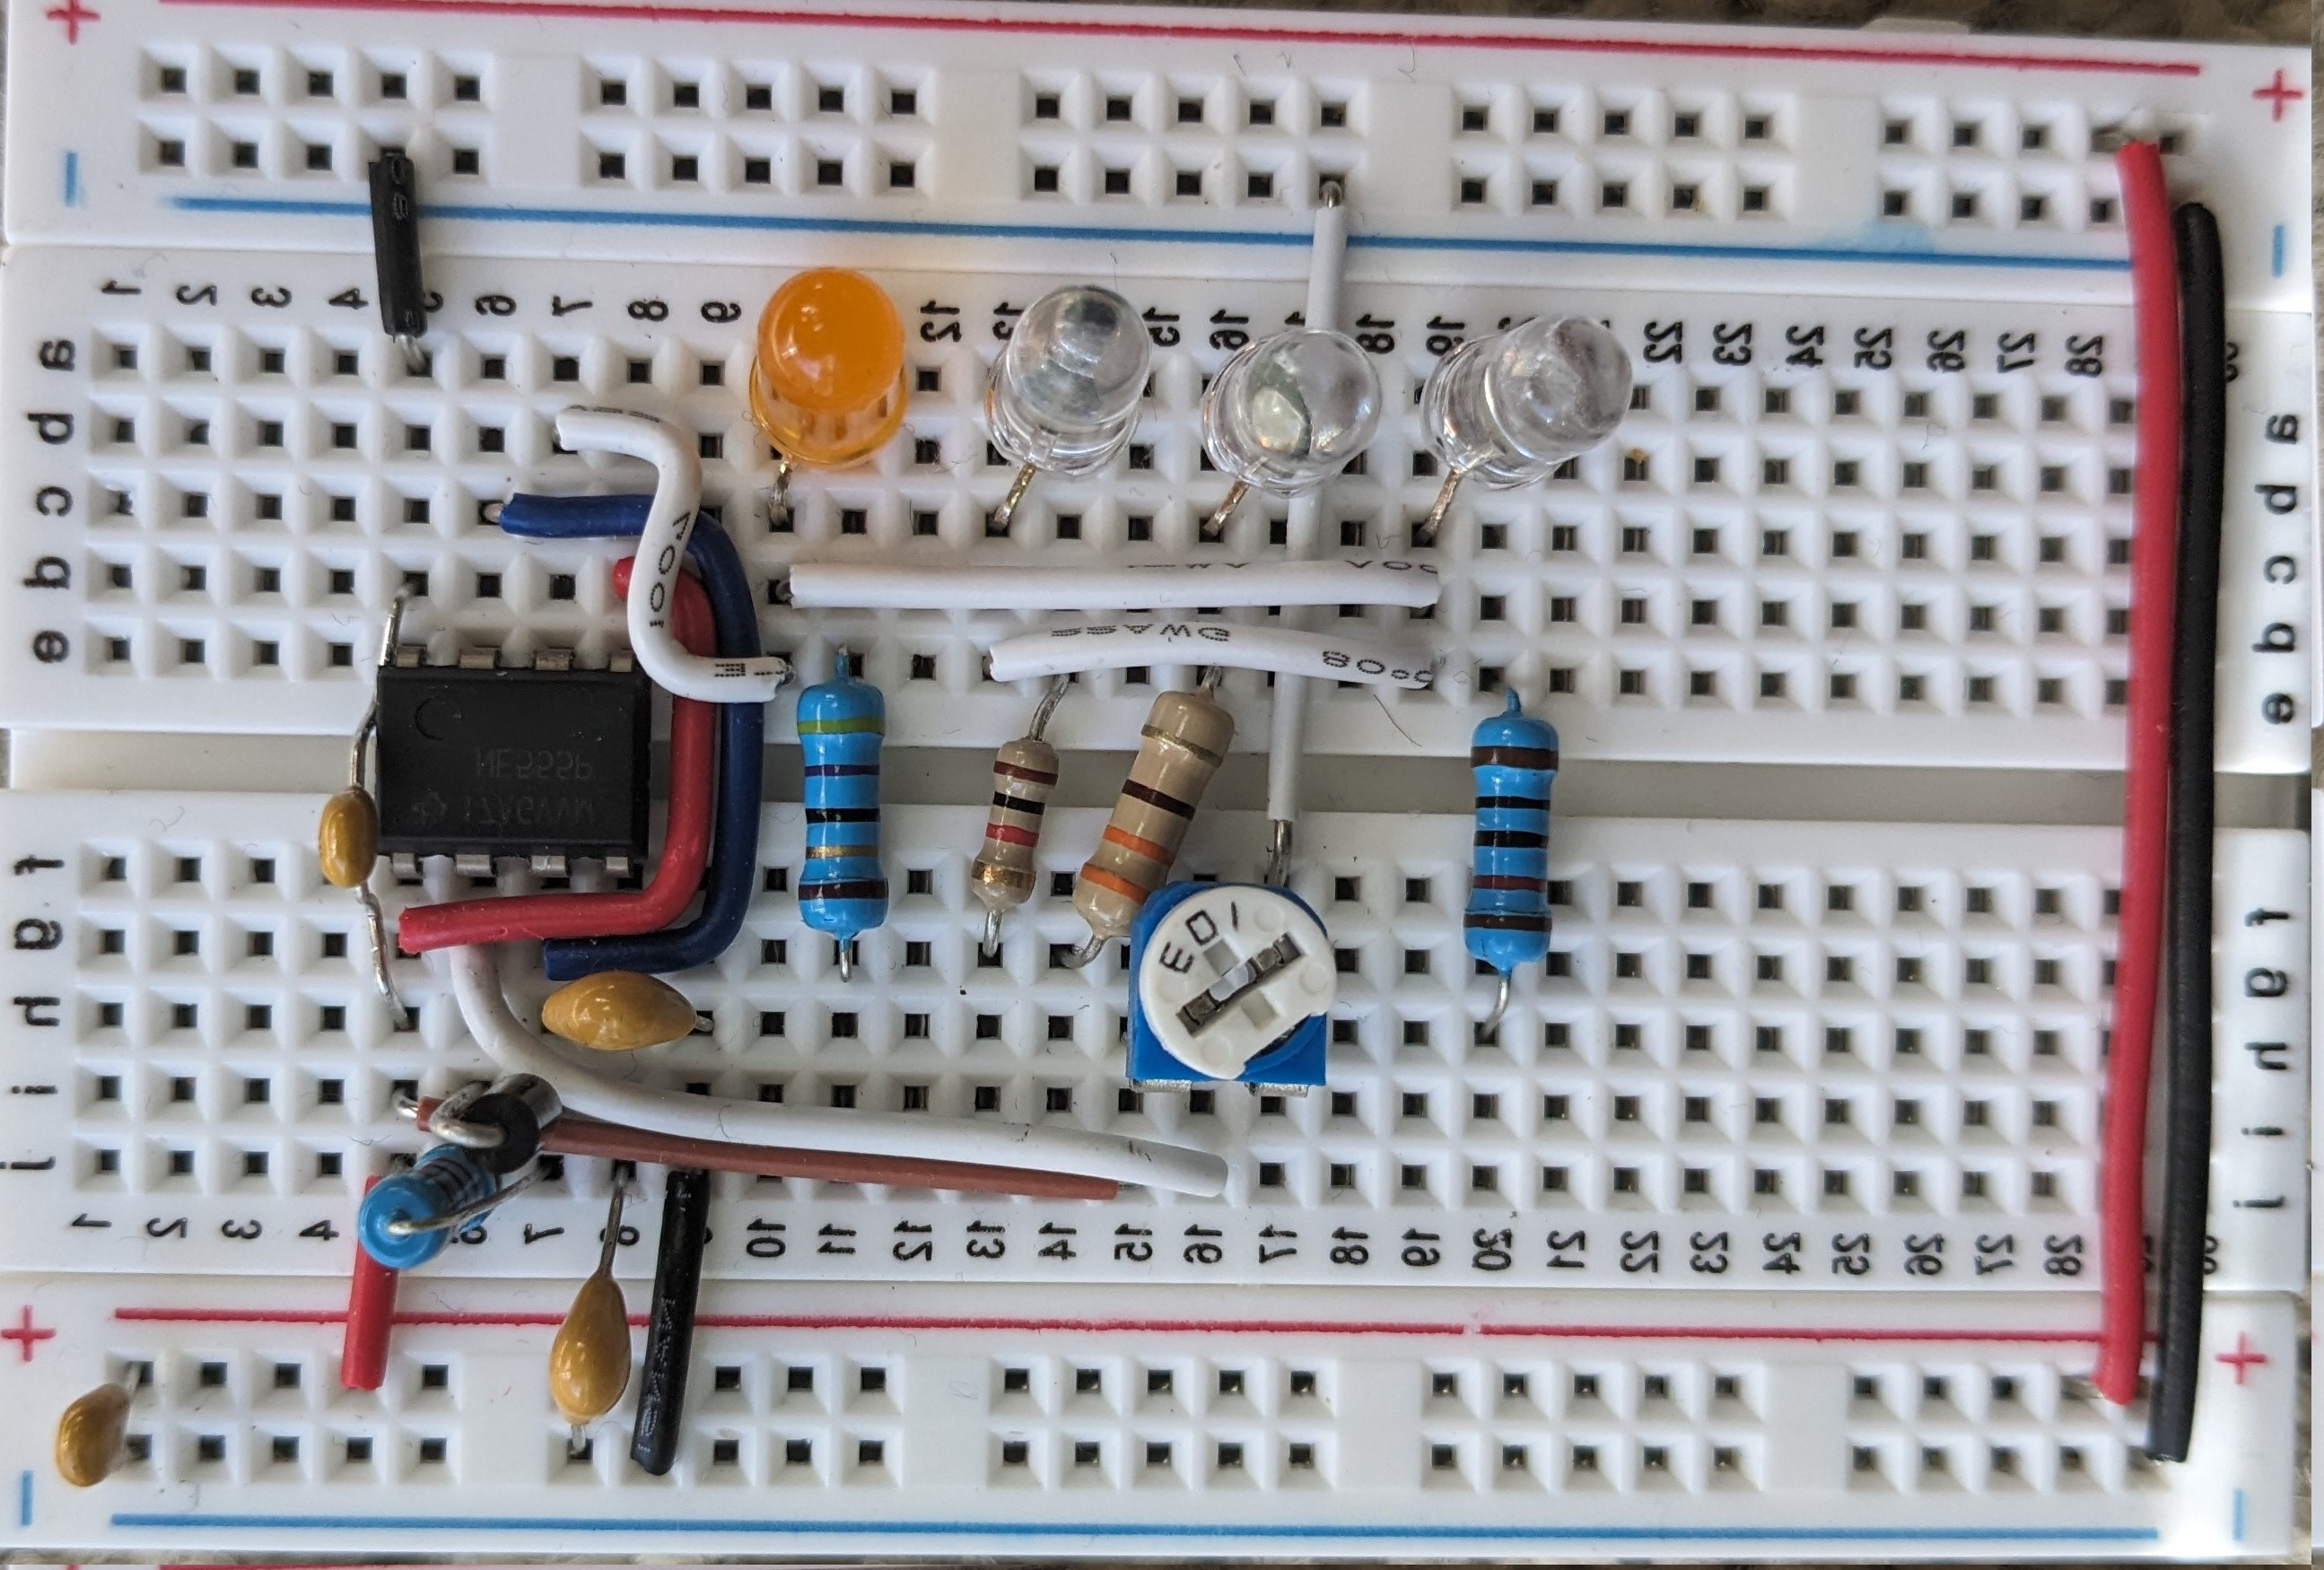
\includegraphics[scale=0.2]{figures/breadboard.jpg}
	\caption{Breadboard Implementation for 555 board}
\end{figure}


\begin{figure}[H]
	\centering
	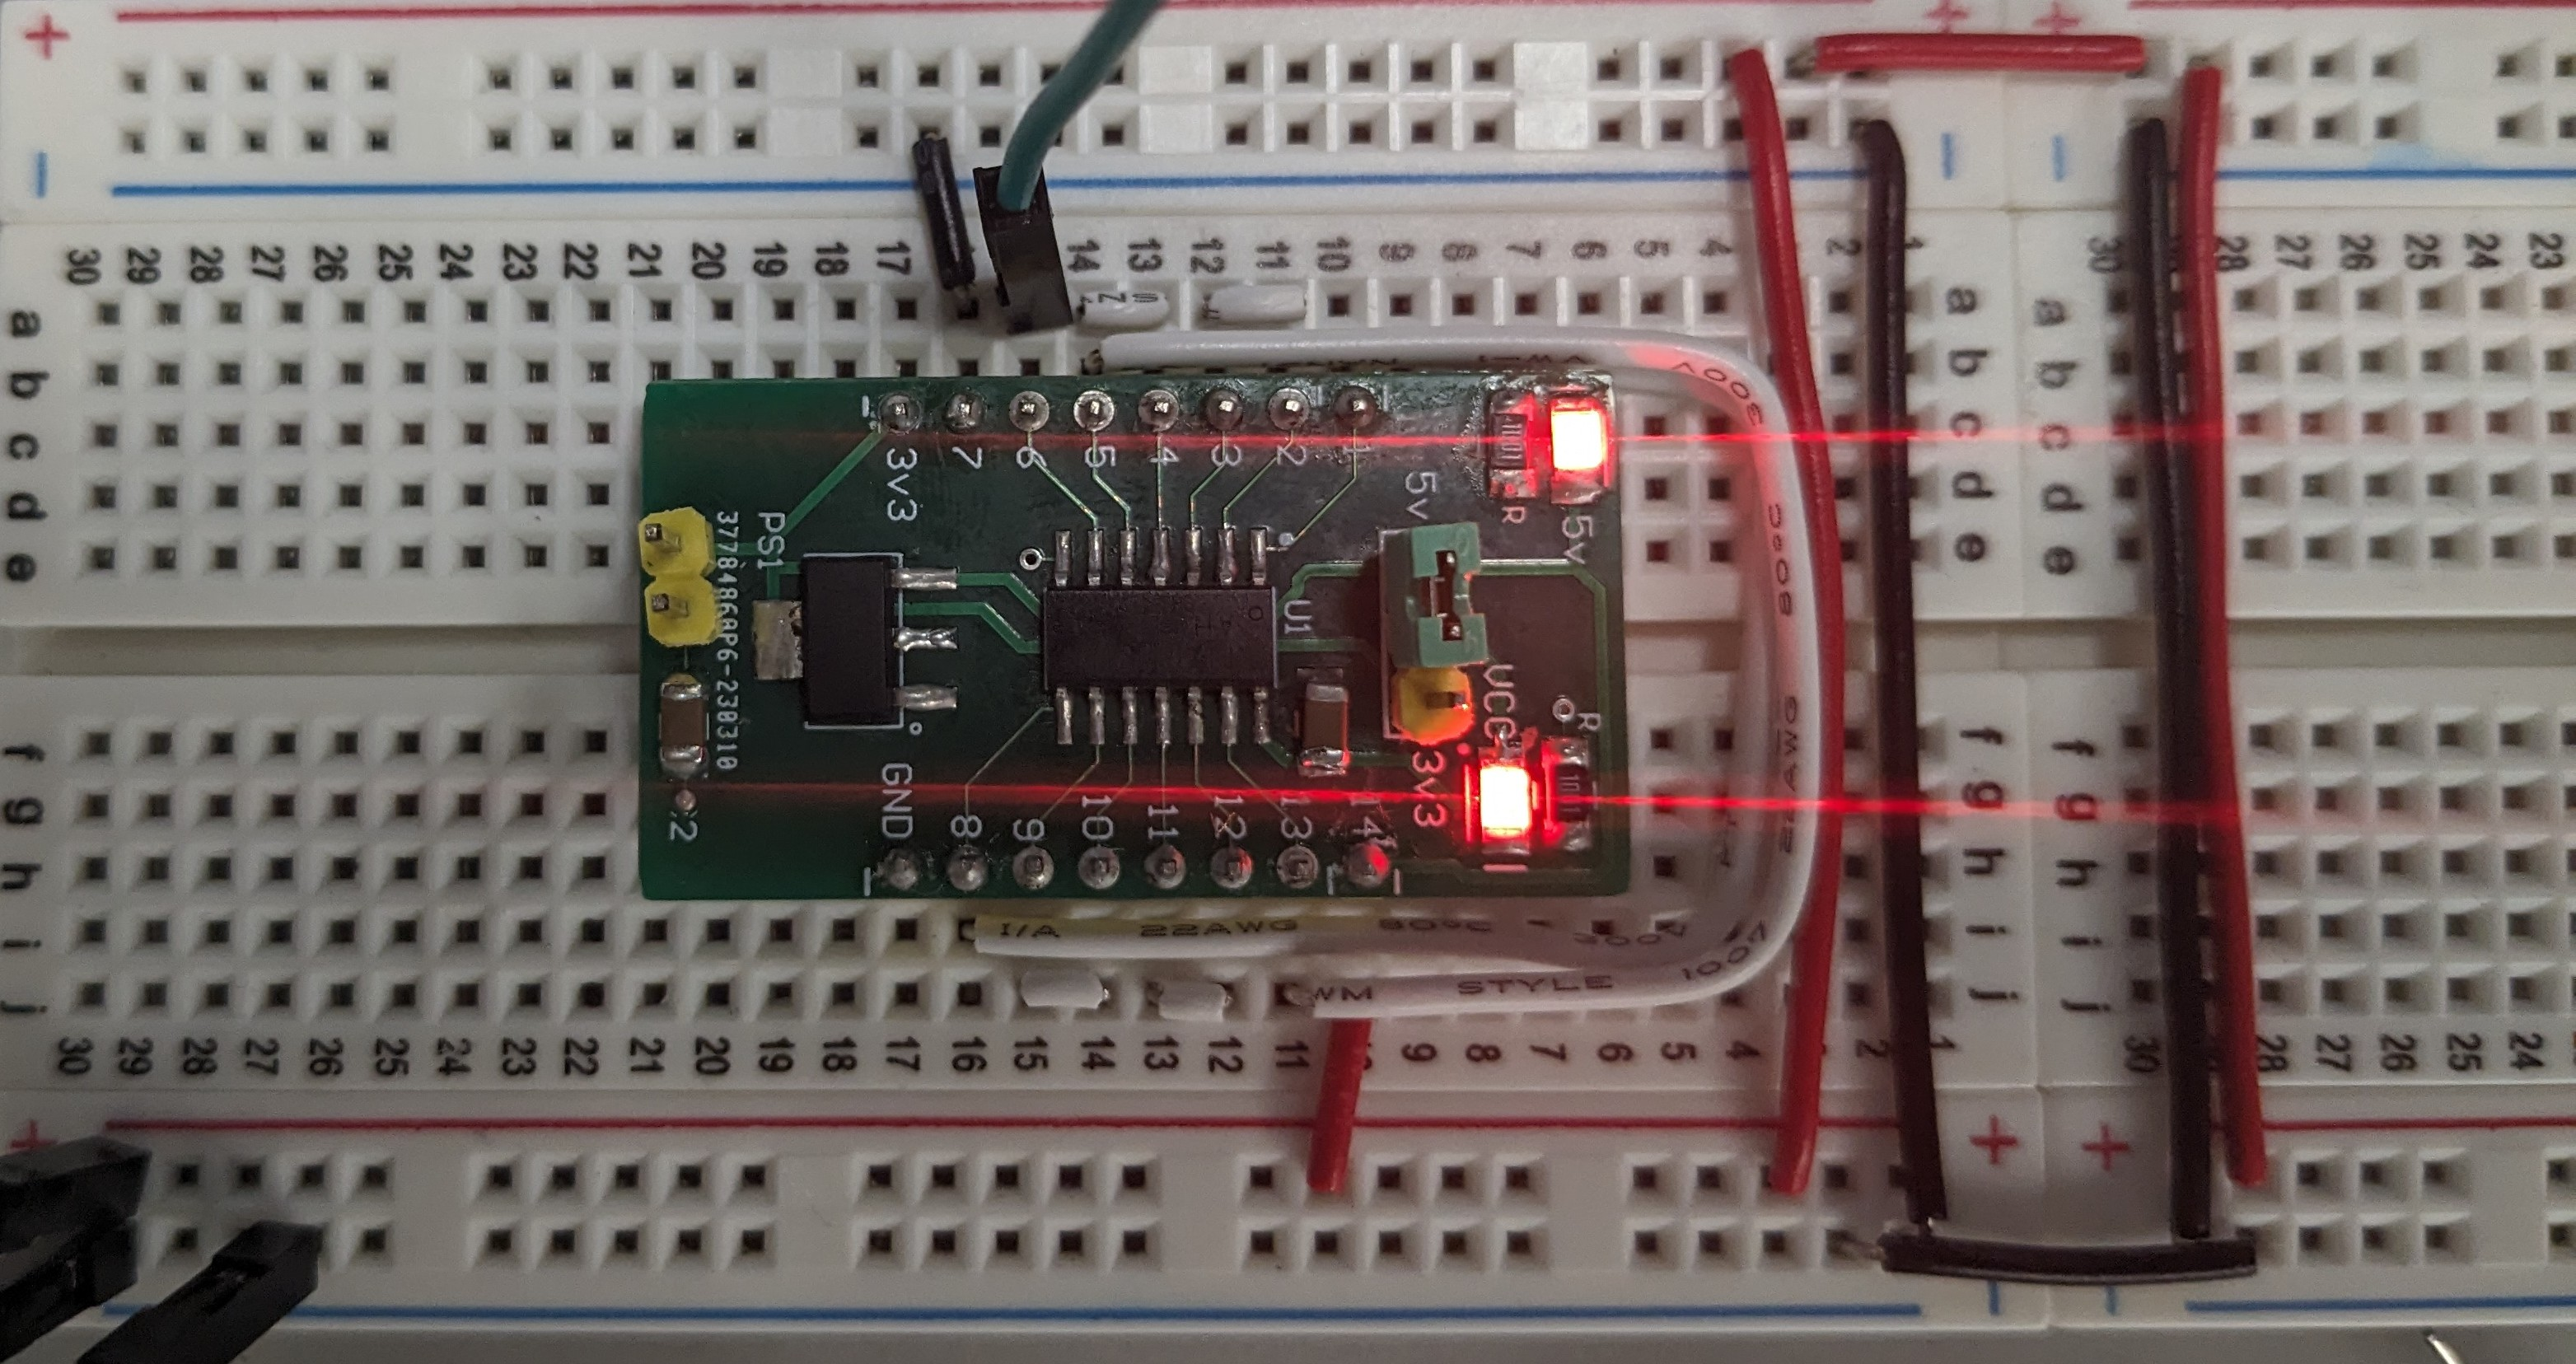
\includegraphics[scale=0.2]{figures/hexboard.jpg}
	\caption{Breadboard Implementation for Hex board}
\end{figure}


The PCB design considerations mentioned should be followed during the manufacturing and assembly process to ensure the final product meets the intended specifications and performs as designed in practical applications.\\

Here is the PCB design:\\

\begin{figure}[H]
	\centering
	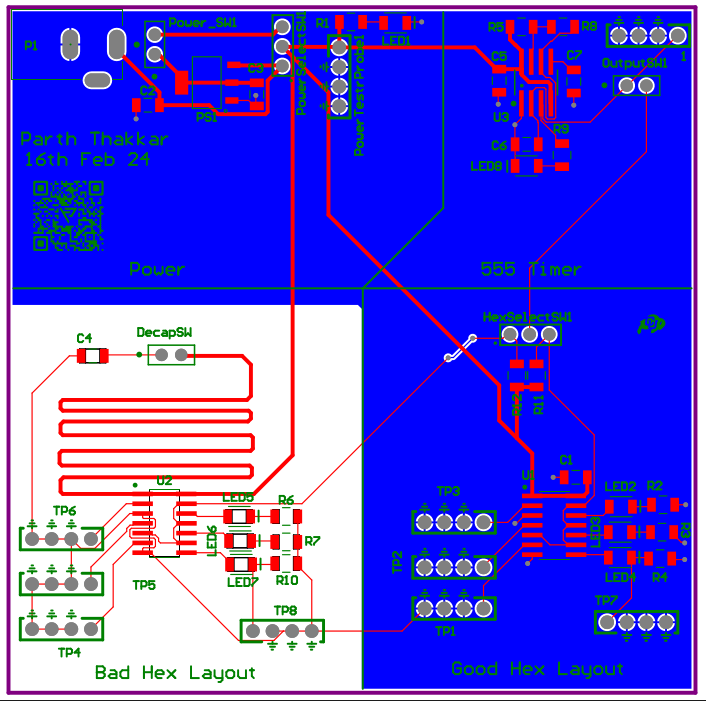
\includegraphics[scale=0.4]{figures/pcb_color.png}
	\caption{Top layer PCB}
	\label{top}
\end{figure}

This is the photo of the PCB after manufacturing\\

\begin{figure}[H]
	\centering
	\includegraphics[scale=0.1]{figures/pcb_.jpg}
	\caption{Manufactured PCB}
\end{figure}

\begin{figure}[H]
	\centering
	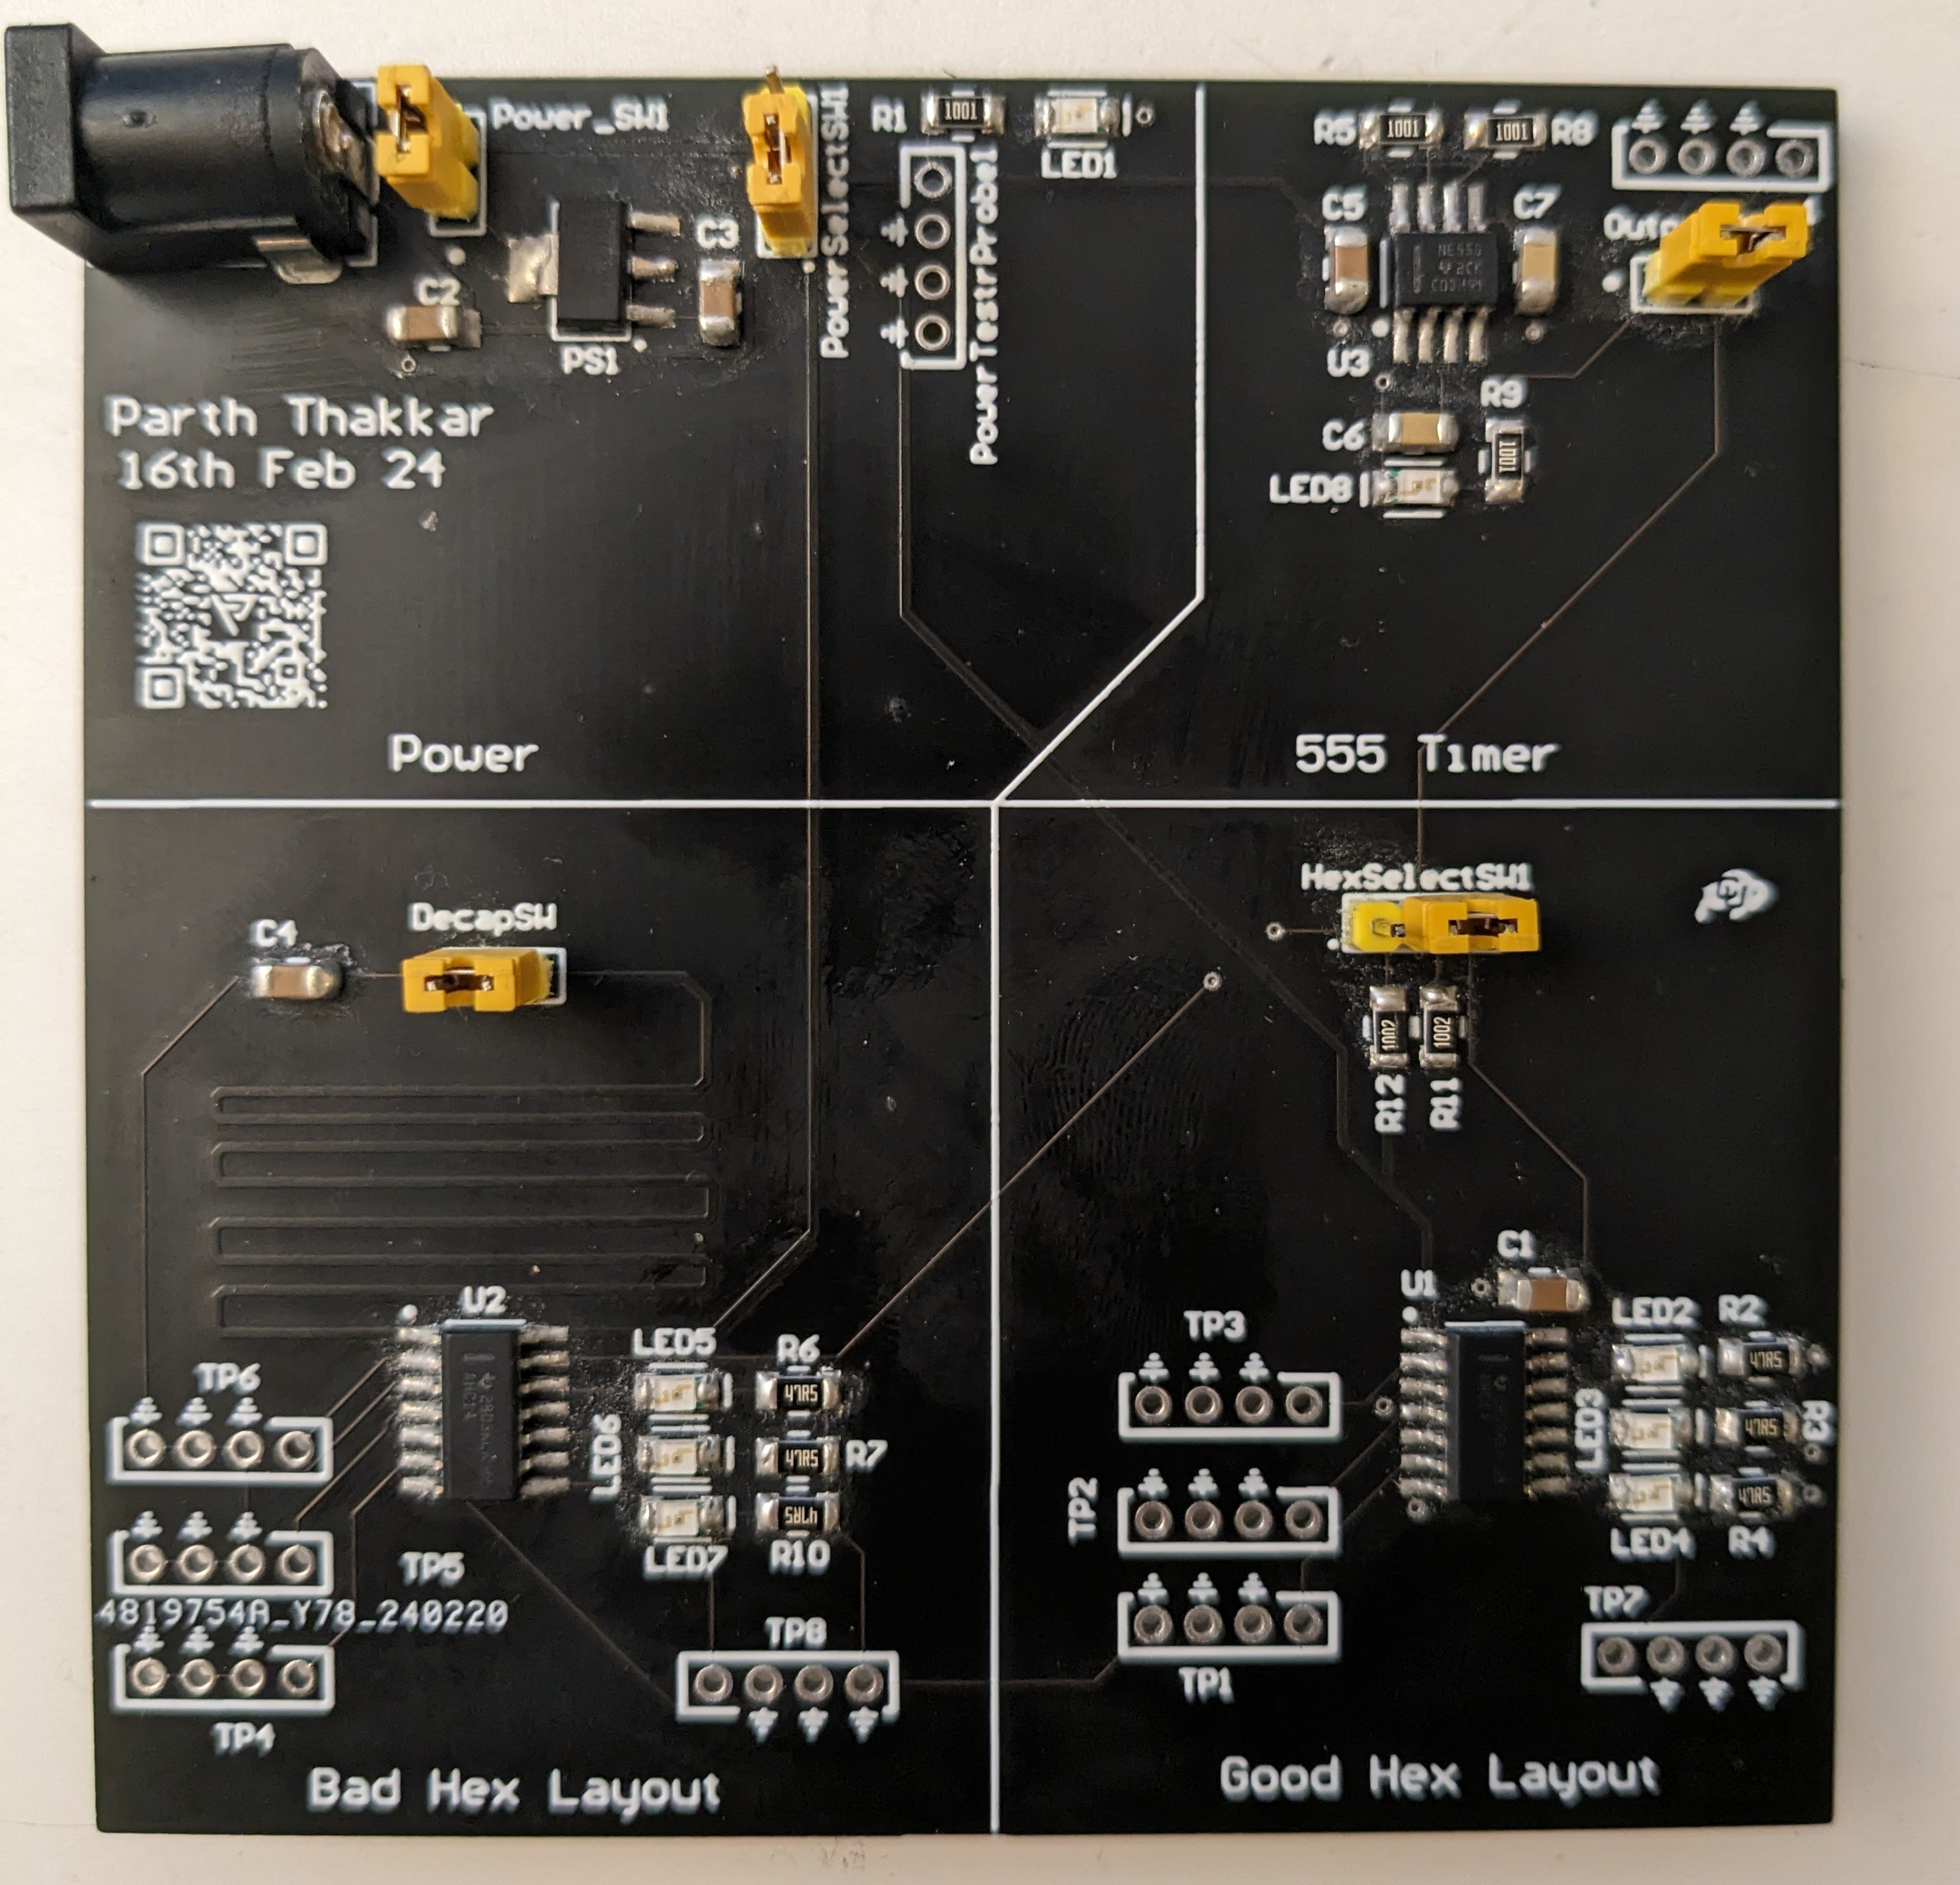
\includegraphics[scale=0.1]{figures/board.jpg}
	\caption{PCB with components soldered}
\end{figure}


\begin{figure}[H]
	\centering
	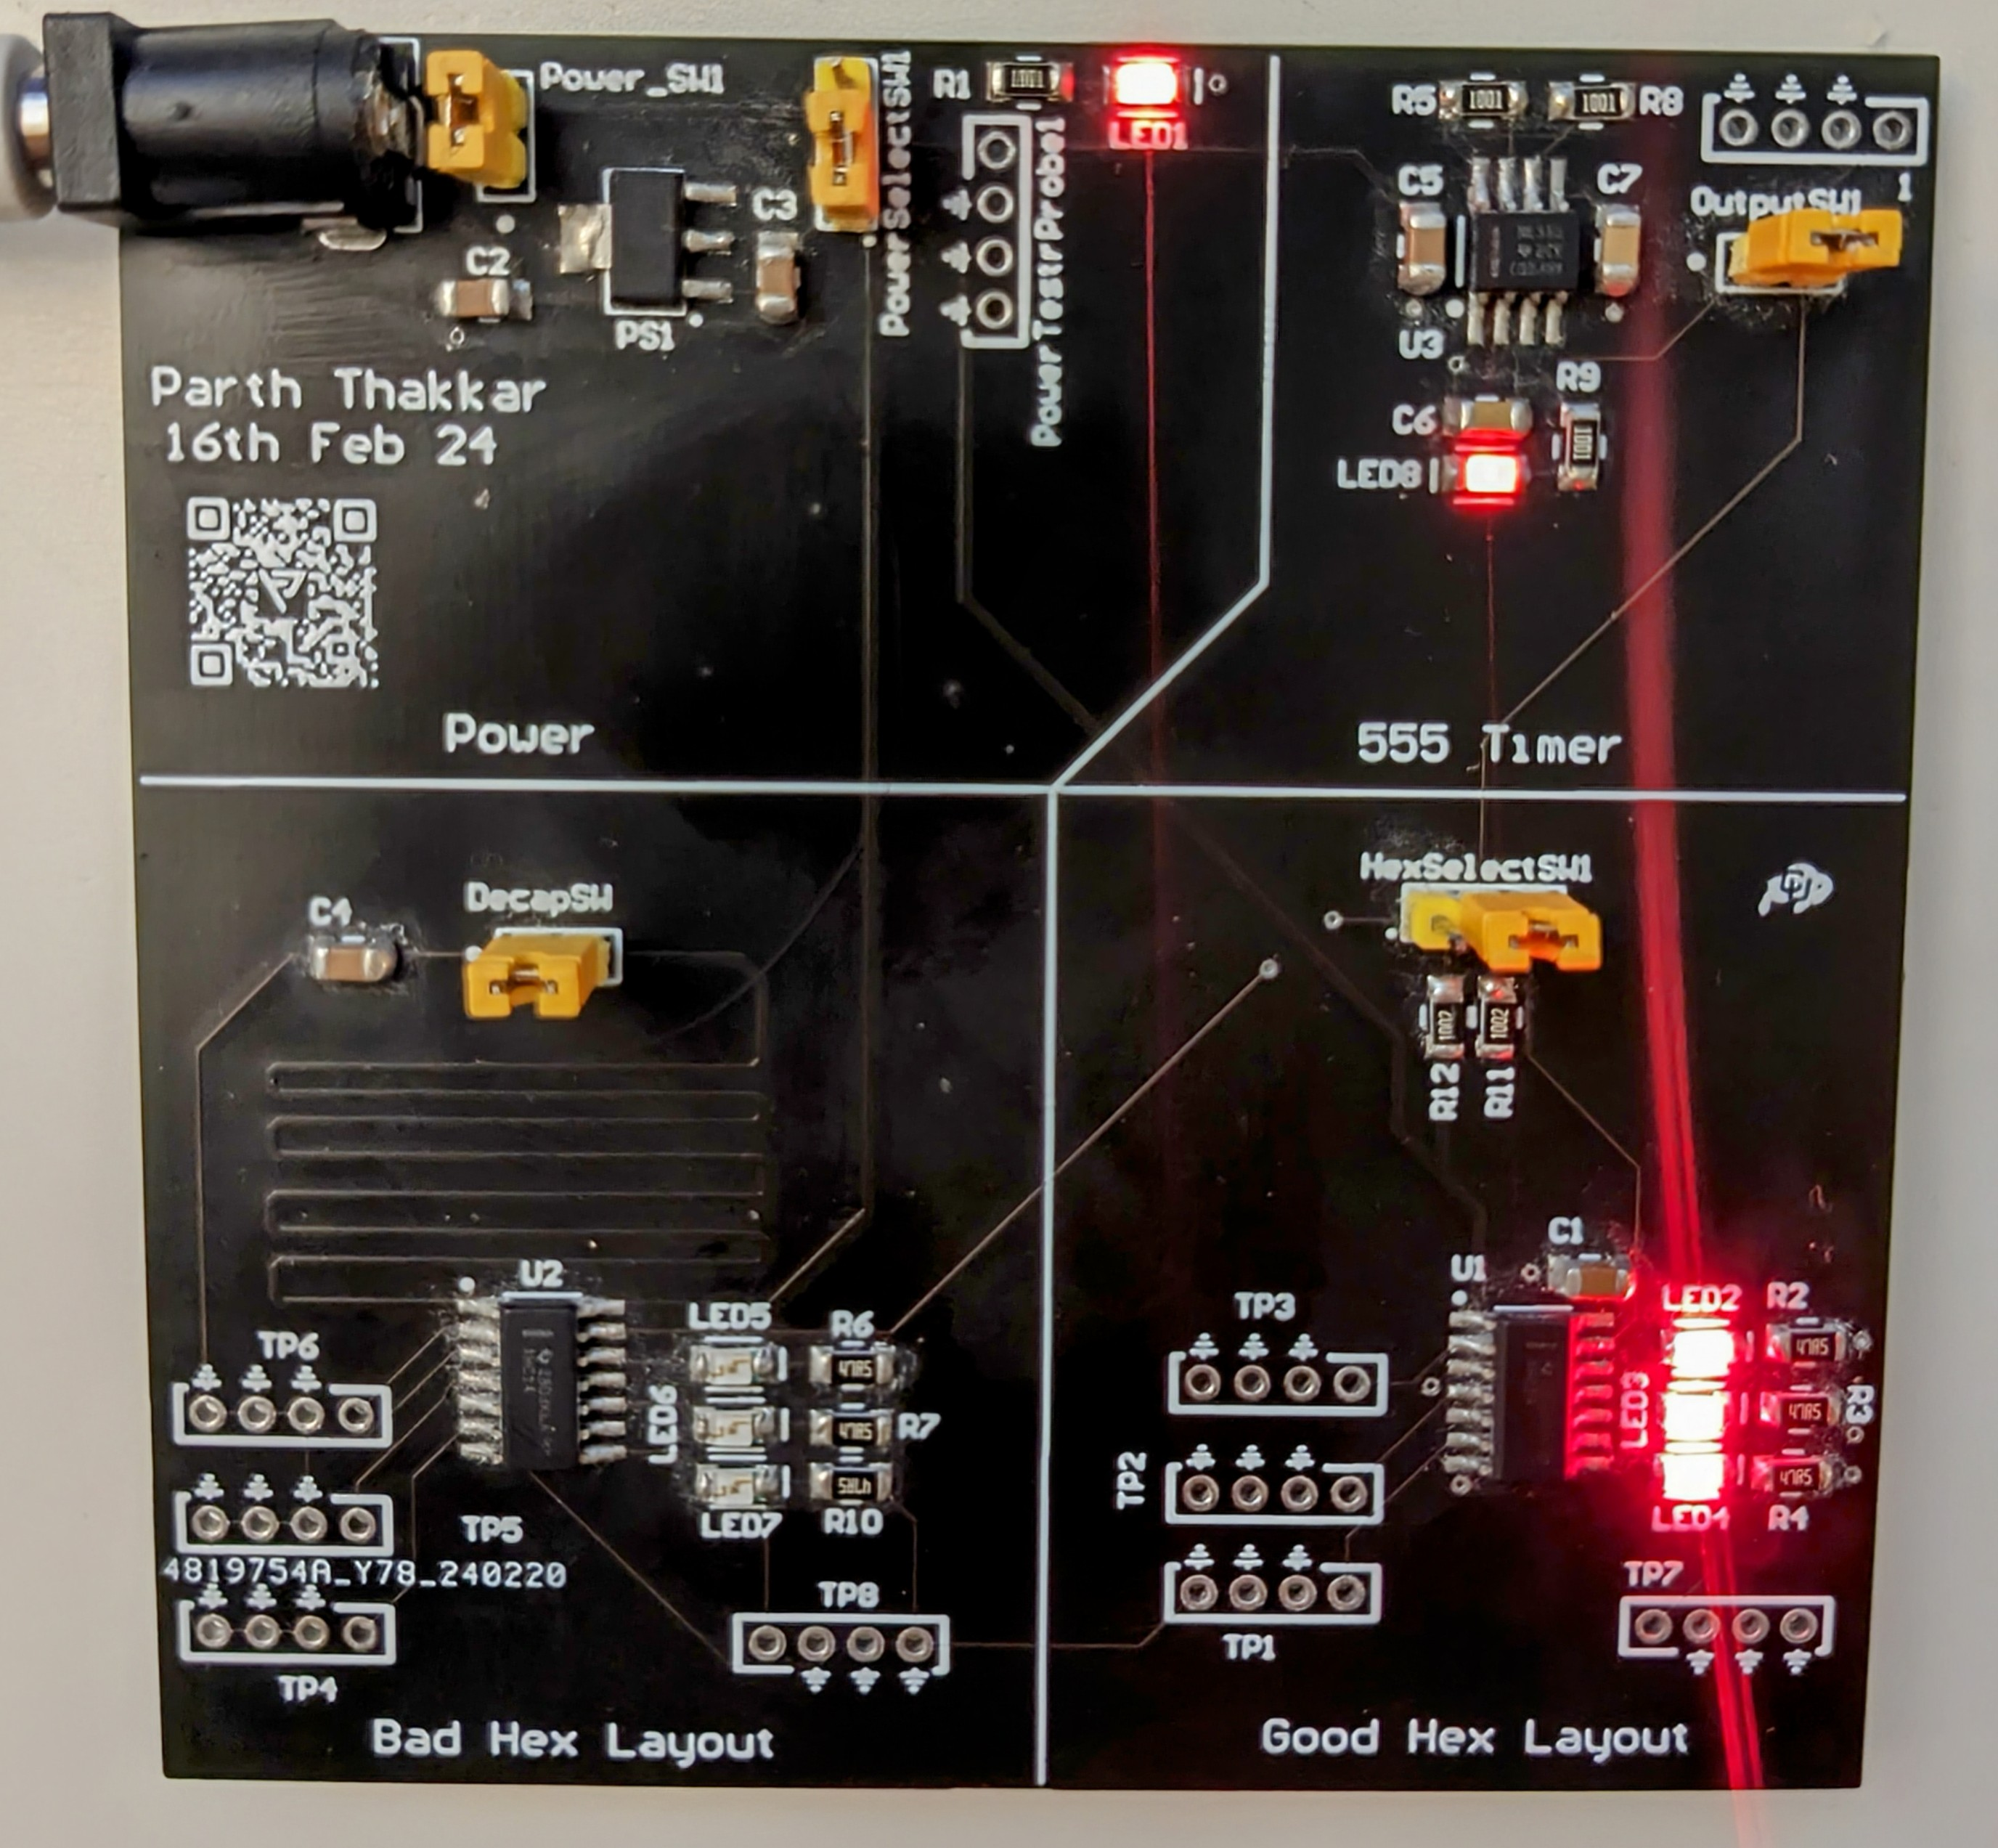
\includegraphics[scale=0.1]{figures/goodpcb.jpg}
	\caption{First time turning on the PCB and selecting good layout}
\end{figure}

\begin{figure}[H]
	\centering
	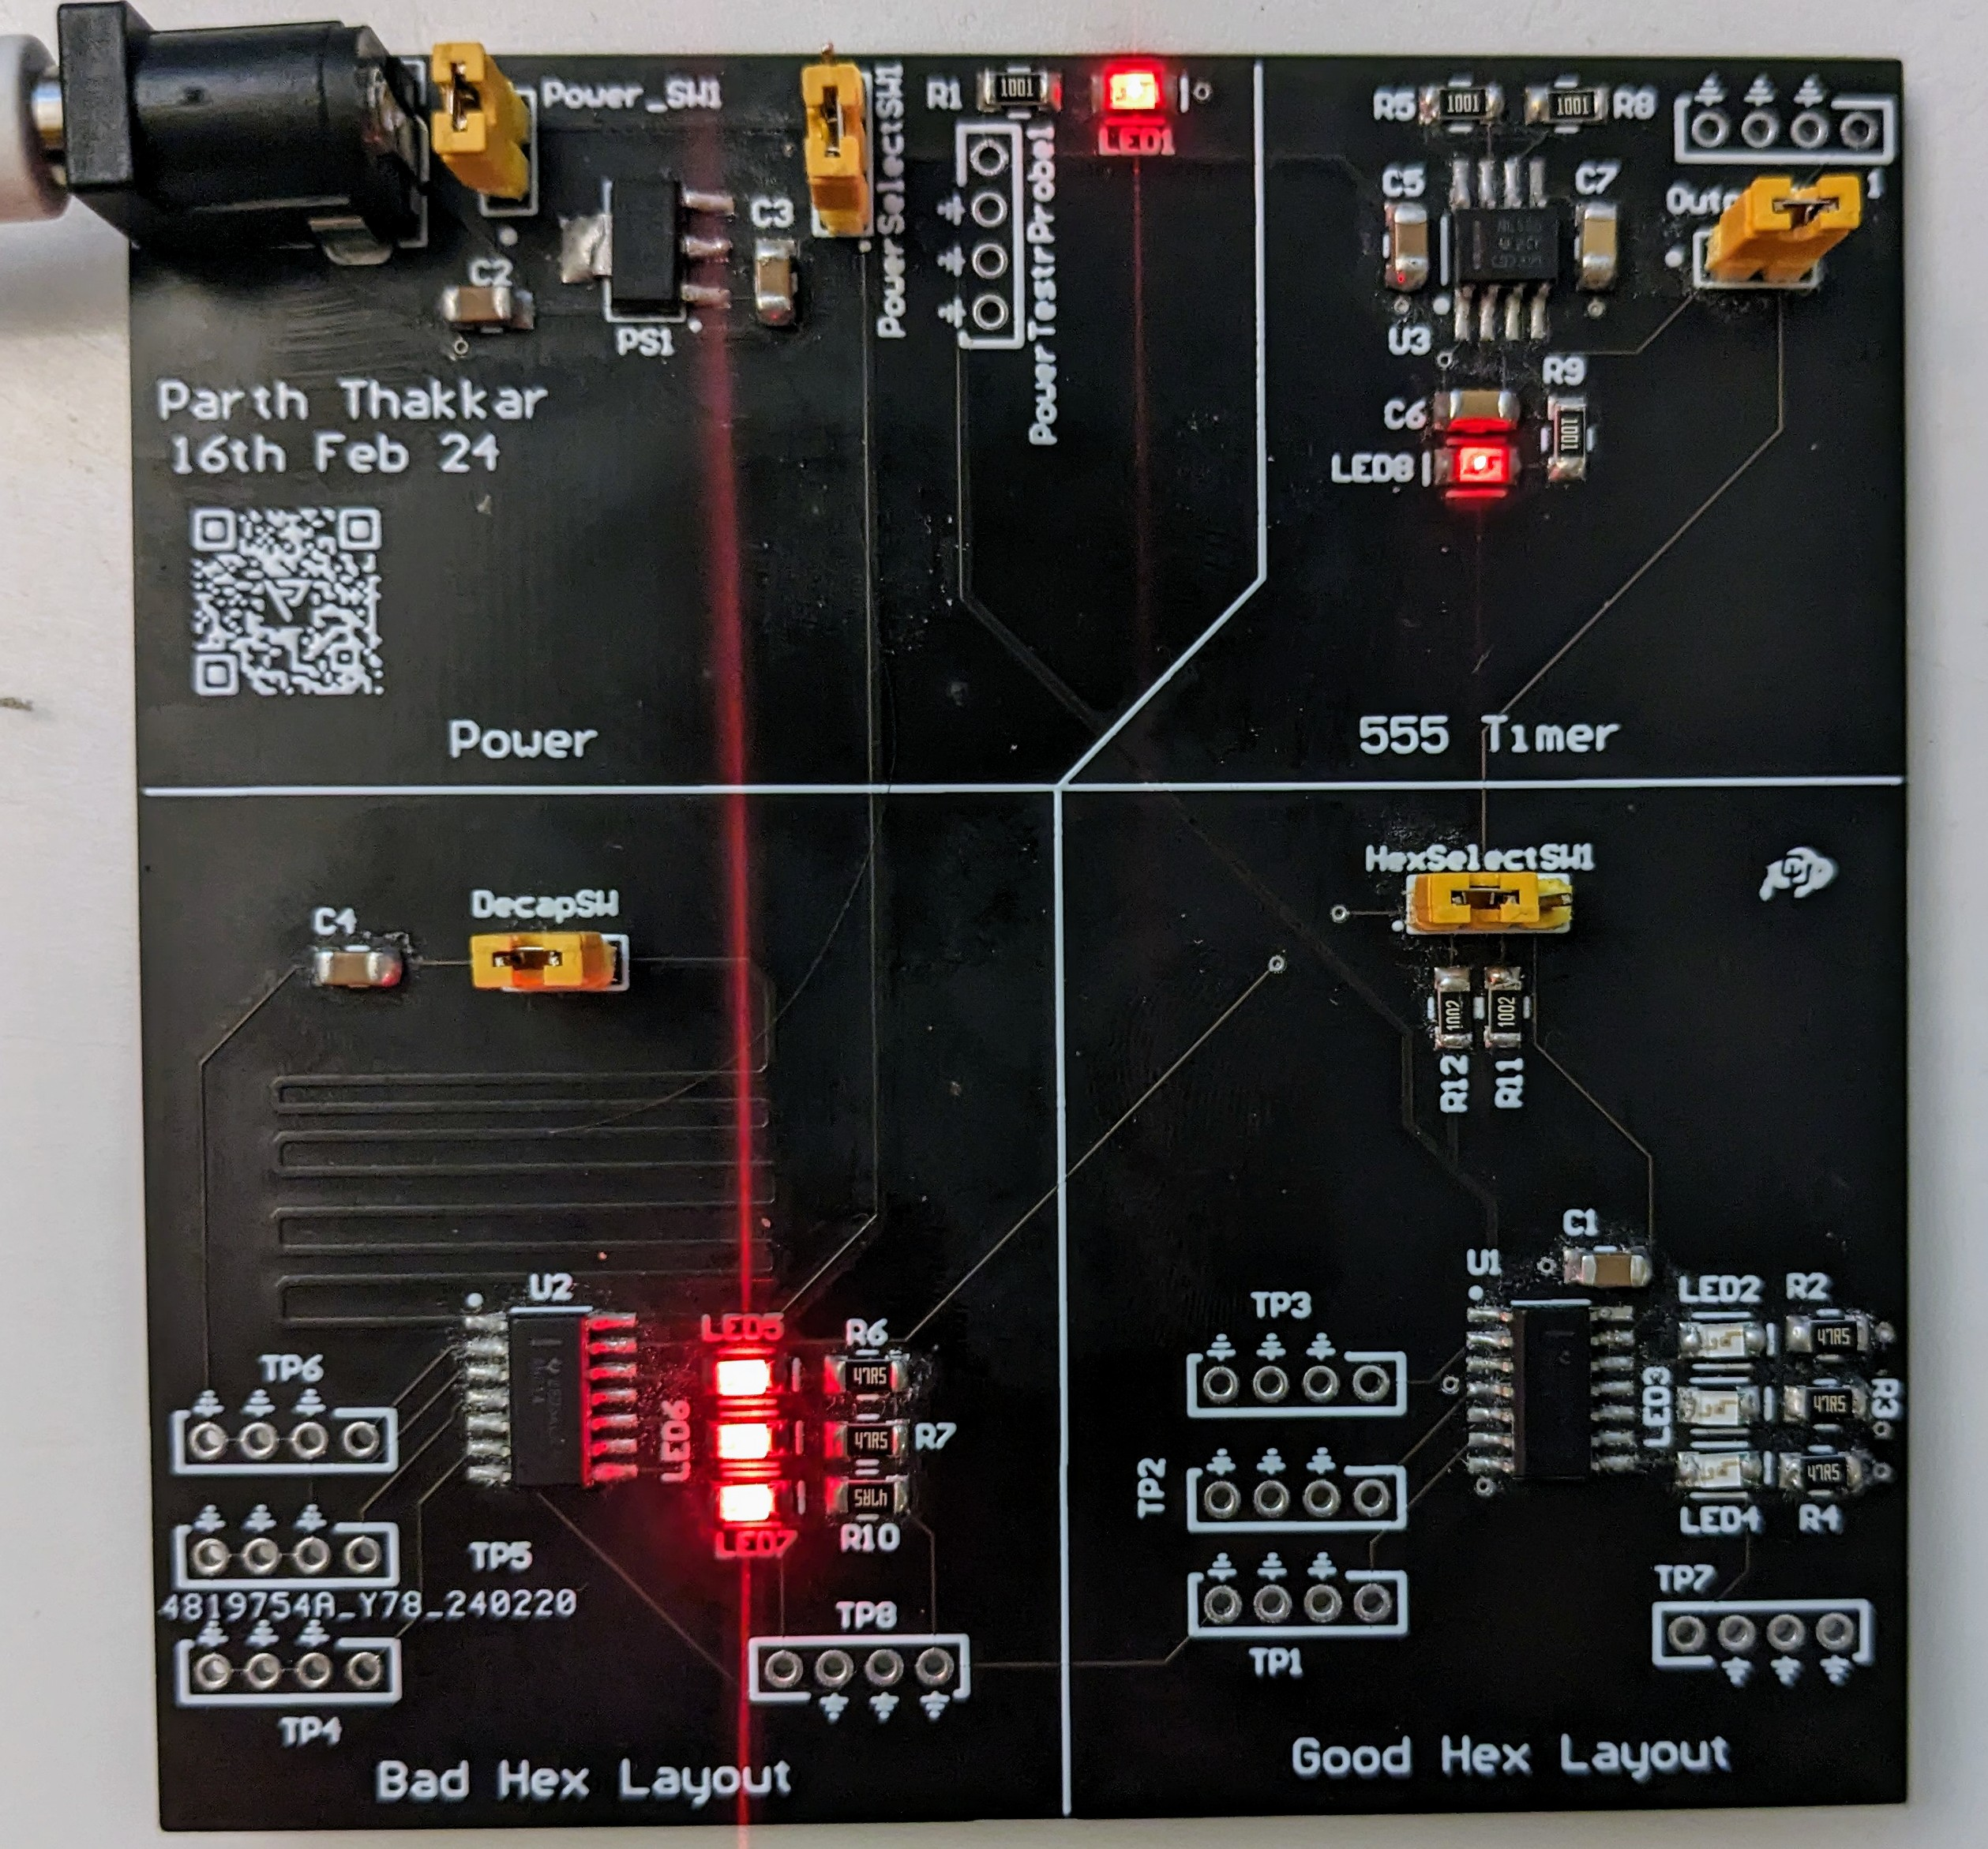
\includegraphics[scale=0.1]{figures/badpcb.jpg}
	\caption{First time turning on the PCB(selecting bad layout)}
\end{figure}

explanation of PCB
\begin{enumerate}
	\item Power Section:
	\begin{itemize}
		\item P1: The power connector, where the external 5V supply is connected to the board.
		\item PS1 and C3: A voltage regulator, a Low Dropout Regulator (LDO) AMS1117, along with its input and output capacitors (C2 and C3) to filter noise from the power supply. This setup steps down the 5V to 3.3V required by the rest of the circuit.
		\item R1 and LED1: These indicate power is being supplied to the board; R1 limits the current to LED1 to prevent it from burning out.
	\end{itemize}
	\item 555 Timer Section:
	\begin{itemize}
		\item U3: The 555 timer IC configured to generate a 500 Hz signal.
		\item R5, R6, R8, R9, C5, C6, and C7: The resistors and capacitors determine the frequency and duty cycle of the 555 timer's output.
		\item OutputSW1 and LED8: A switch and an LED used to enable/disable and indicate the output of the 555 timer.
	\end{itemize}
	\item Good Hex Inverter Layout:
	\begin{itemize}
		\item U1: A hex inverter IC with a good layout, meaning it has a clean and organized routing of traces and proper placement of components to minimize noise and interference.
		\item C1: The decoupling capacitor placed close to the VCC pin of U1 to filter out noise and provide a stable voltage supply.
		R2, R4, LED2, LED4: Resistors and LEDs connected to the outputs of the hex inverter to serve as loads and visual indicators of the inverter’s output.
		\item TP1, TP2, TP3: Test points for probing the power supply and the outputs of the good hex inverter.
		\item HexSelectSW1: A switch to select different outputs of the hex inverter.
	\end{itemize}
	\item Bad Hex Inverter Layout:
	\begin{itemize}
		\item 	U2: Another hex inverter IC, but laid out with suboptimal design practices, which may include longer trace lengths and poor decoupling practices.
		\item C4 (DecapSW): The decoupling capacitor for U2, intentionally placed far from the VCC pin to demonstrate the effects of a bad layout.
		\item R7, R10, LED7, LED9: Similar to the good layout, these components serve as loads and indicators for the outputs of U2.
		\item TP4, TP5, TP6: Test points to analyze the outputs and power supply to U2.
	\end{itemize}

	\item LDO and Plane Routes:
	\begin{itemize}
		\item The LDO (low-dropout regulator) is represented by PS1 and C3, providing the regulated 3.3V power supply.
		\item Plane routes refer to the large areas of copper on the PCB, which are used for power distribution (ground planes).
	\end{itemize}
	
\end{enumerate}



\section{Calculations for Duty Cycle and Frequency}


We need out circuit to produce around 50\% duty cycle with 500Hz of frequency.

\begin{enumerate}
	\item for simple circuit we can see that the overall time for one cycle would be\\
	\begin{flalign*}
		& T_{total} = T_{charging} + T_{discharging}&& \\\\
		& \textbf{And expanding each timing term would give us,}&& \\
		&T_{charging} = 0.693 \cdot(R_1 + R_2) \cdot C&& \\
		& T_{discharging} = 0.693 \cdot(R_2) \cdot C&& \\\\
		&\textbf{so the total time for charging and Discharging would be, }&& \\
		&T_{total} = 0.693 \cdot(R_1 + R_2) \cdot C + 0.693 \cdot(R_2) \cdot C&& \\
		&T_{total} = 0.693 \cdot(R_1 +  2 \cdot R_2) \cdot C&& \\
	\end{flalign*}
	\item Adding components to the circuit:\\
	
	\begin{flalign*}
	&T_{charging} = 0.693 \cdot(R_1 +  R_2) \cdot C&& \\
	&T_{discharging} = 0.693 \cdot (R_2) \cdot C&& \\\\
	&T_{total} = 0.693 \cdot(R_1 + 2 \cdot R_2) \cdot C&& \\
	&T_{total} = 0.693 \cdot(1000 + 2000) \cdot 1 \cdot 10^{-6}&& \\
	&T_{total} = 2079 \cdot 10^{-6}&& \\
	&f_{total} = \frac{1}{T_{total}}&& \\
	&\boxed{f_{total} = 481 Hz}&& \\
	\end{flalign*}
	
	And duty cycle would be 66.67\%.

	
\end{enumerate}

\section{Output Waveforms / Measurement}

\subsection{Power Rail 5V Measurement:}

\begin{itemize}
	\item Objective: Confirm that the input power supply is at the desired 5V level.
	\item 
	\begin{figure}[H]
		\centering
		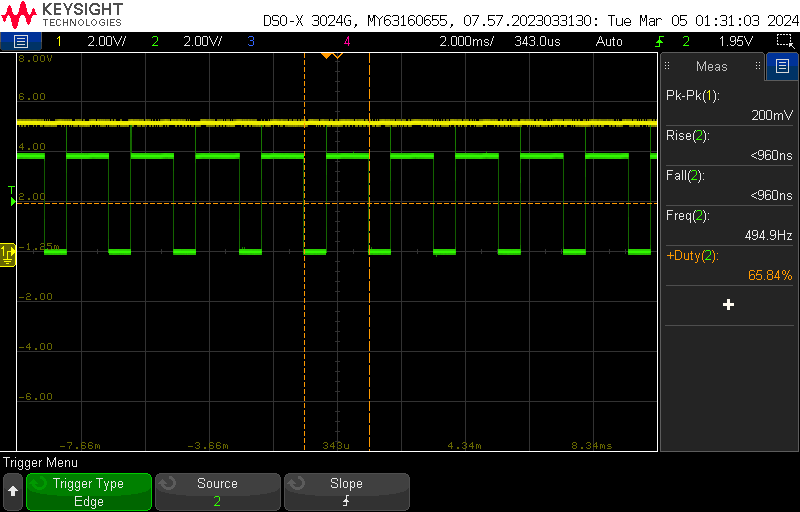
\includegraphics[scale=0.6]{figures/scope_0.png}
		\caption{Fall time with load connected}
		\label{scope_0}
	\end{figure}
	\item Results: Input power rail measurement confirming a stable 5V supply.
\end{itemize}


\subsection{Bad Layout Analysis:}
\begin{enumerate}
	\item Objective: Understand why the 'bad' layout yields poor performance.
	\item Why is is 'bad'
	\begin{itemize}
		\item Absence of return planes.
		\item Decoupling capacitor placed far from the IC.
		\item Long and closely placed tracks.
	\end{itemize}
	\item Results:  Such design practices lead to increased switching noise from the PDN and signal-return paths.
\end{enumerate}

\subsubsection{Bad Layout Output Measurements:}

\begin{enumerate}
	\item 
	Rise Time Measurement:
	\begin{itemize}
		\item Objective: Measure the rise time affected by rail noise.
		\item 
		\begin{figure}[H]
			\centering
			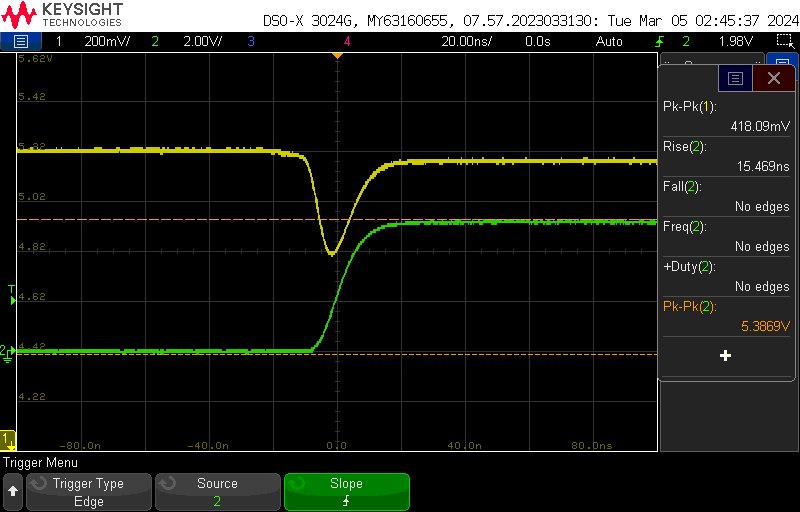
\includegraphics[scale=0.6]{figures/bad/quite_high/rise/rising_qh_bad4.png}
			\caption{Fall time with load connected}
		\end{figure}
		\item Results: The rise time of 15.469 ns, indicating longer rise time due to more noise in bad layout.
	\end{itemize}
	
	\item Fall Time Measurement:
	\begin{itemize}
		\item Objective: Measure the fall time of the scope trigger signal.
		\item 
		\begin{figure}[H]
			\centering
			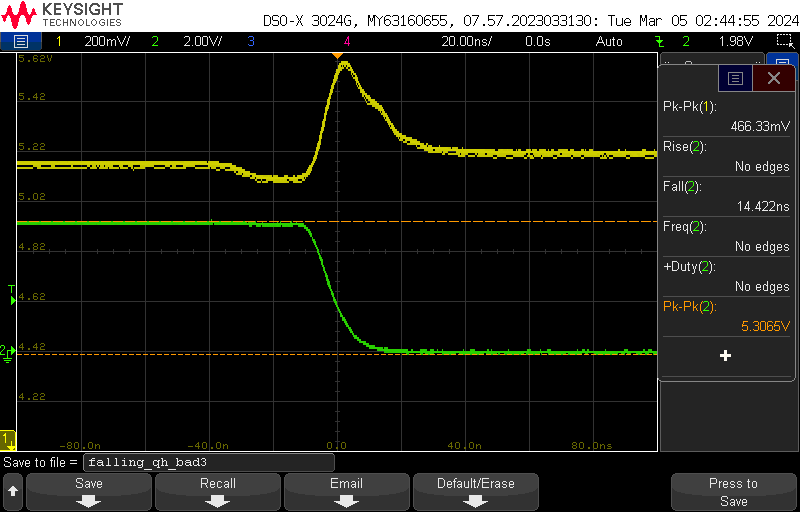
\includegraphics[scale=0.6]{figures/bad/quite_high/fall/falling_qh_bad3.png}
			\caption{Fall time with load connected}
		\end{figure}
		
		\item Results: Fall time of 14.422 ns in the bad layout.
	\end{itemize}
	
\end{enumerate}



\subsubsection{Bad Layout Noise Measurement:}

\begin{enumerate}
	\item Noise at Quiet High (Rise/Fall):
	\begin{itemize}
		\item Objective: Quantify switching noise at quiet high during rise and fall.
		\item 
		\begin{figure}[H]
			\centering
			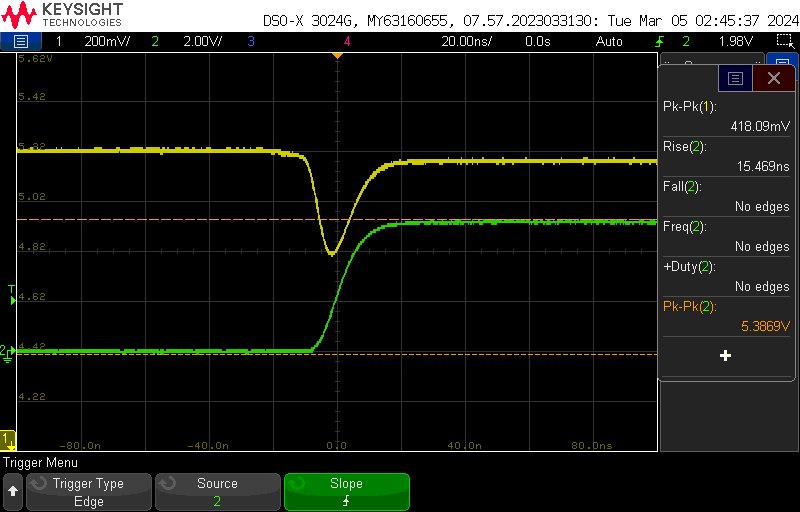
\includegraphics[scale=0.6]{figures/bad/quite_high/rise/rising_qh_bad4.png}
			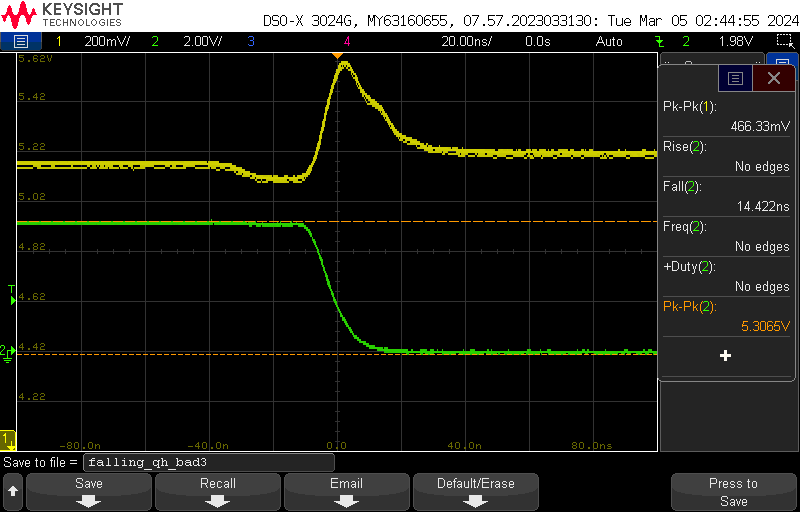
\includegraphics[scale=0.6]{figures/bad/quite_high/fall/falling_qh_bad3.png}
			\caption{Bad layout Quite high Rise \& Fall time with load connected}
		\end{figure}

		
		\item Results:\\
		Noise measured at 418.09 mV with a rise time of 15.468 ns.\\
		Noise measured at 466.33 V with a fall time of 14.422 ns.
	\end{itemize}

	\item Noise at Quiet Low (Rise/Fall):
	\begin{itemize}
		\item Objective: Quantify switching noise at quiet low during rise and fall.
		\item 
		\begin{figure}[H]
			\centering
			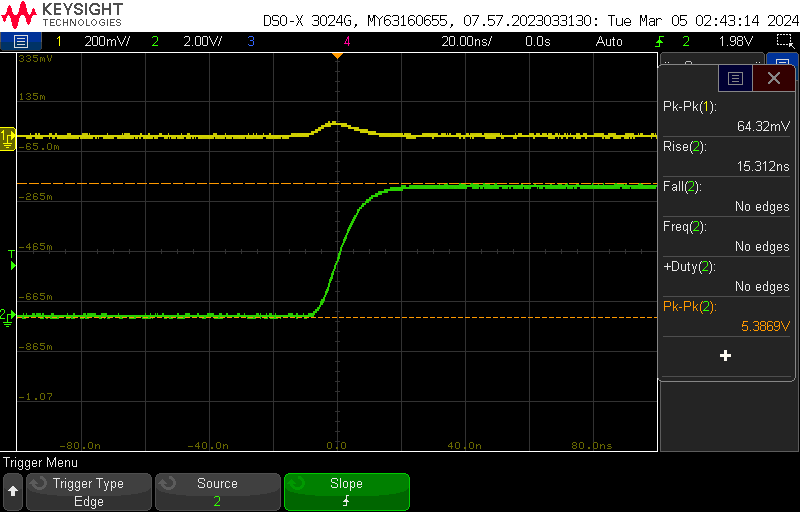
\includegraphics[scale=0.6]{figures/bad/quite_low/rise/rising_ql_bad1.png}
			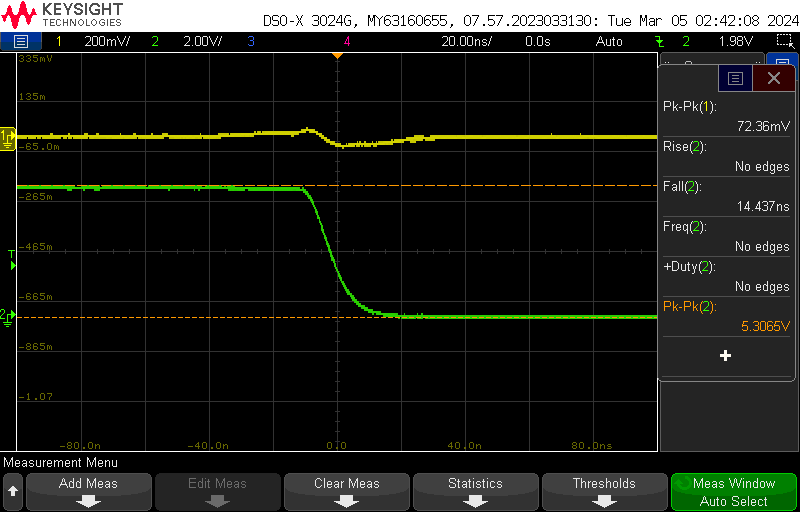
\includegraphics[scale=0.6]{figures/bad/quite_low/fall/falling_ql_bad.png}
			\caption{Bad layout Quite Low Rise \& Fall time with load connected}
		\end{figure}
		\item Results:\\
		Noise measured at 64.32 mV with a rise time around 15 ns.\\
		Noise measured at 72.36 mV with a fall time around 14.4 ns.\\
	\end{itemize}
	
	
\end{enumerate}


\subsection{Good Layout Analysis:}
\begin{enumerate}
	\item Objective: Present the advantages of a 'good' layout for reducing switching noise.
	\item Highlights of Good Design:
	\begin{itemize}
		\item Presence of a common return plane.
		\item Decoupling capacitor placed close to the IC.
		\item Short tracks.
	\end{itemize}
	
\end{enumerate}



\subsubsection{Good Layout Output Measurements:}
\begin{enumerate}
	\item Rise Time Measurement:
	\begin{itemize}
		\item Objective: Compare the rise time with that of the bad layout.
		\item 
		\begin{figure}[H]
			\centering
			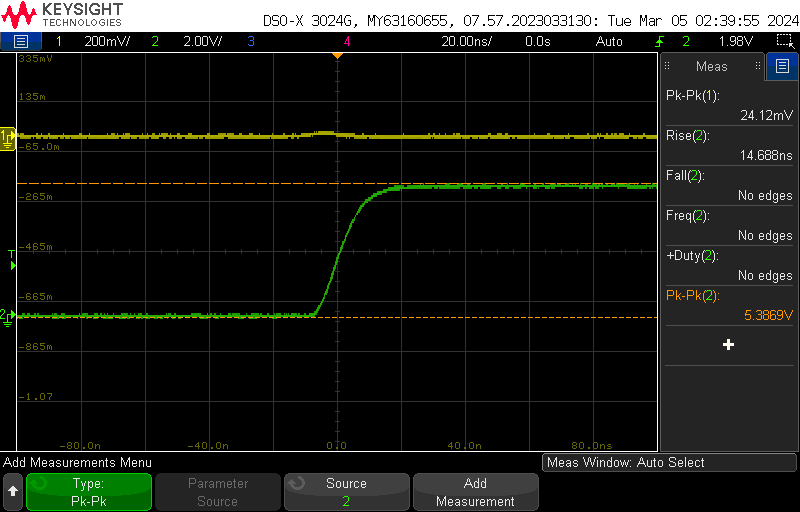
\includegraphics[scale=0.6]{figures/good/quite_low/rise/rising_good_low.png}
			
			
		\end{figure}
		\item Results: Faster rise time of 14.688 ns due to good design practices.
	\end{itemize}
	
	\item Fall Time Measurement:
	\begin{itemize}
		\item Objective: Compare the fall time with that of the bad layout.
		\item 
		\begin{figure}[H]
			\centering
			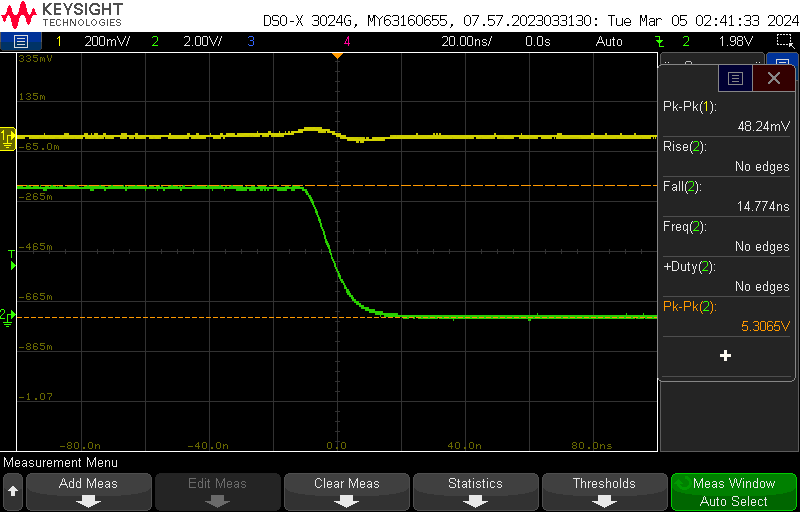
\includegraphics[scale=0.6]{figures/good/quite_low/fall/falling_ql_good.png}
		\end{figure}
		\item Results: Fall time of 14.7 ns, showing improvement over the bad layout.
	\end{itemize}
	
\end{enumerate}

\subsubsection{Good Layout Noise Measurement:}

\begin{enumerate}
	\item Noise at Quiet High (Rise/Fall):
	\begin{itemize}
		\item Objective: Measure and compare the switching noise at quiet high with the bad layout.
		\item 
		\begin{figure}[H]
			\centering
			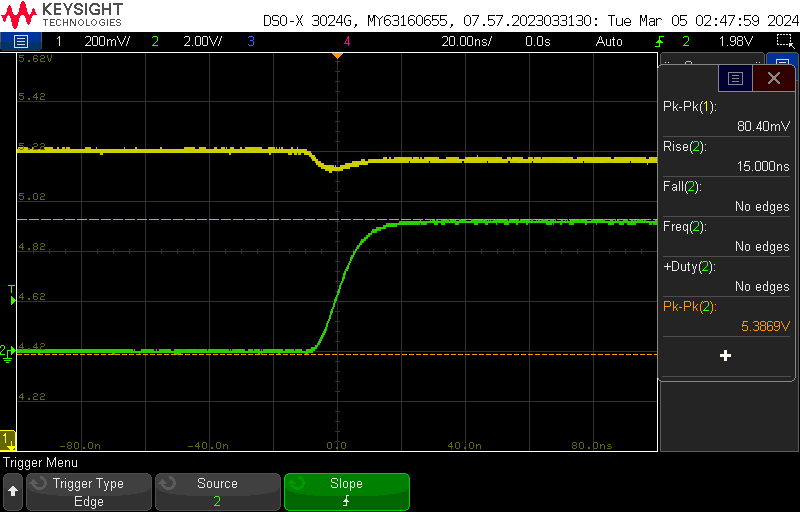
\includegraphics[scale=0.6]{figures/good/quite_high/rise/rising_qh_good7.png}
			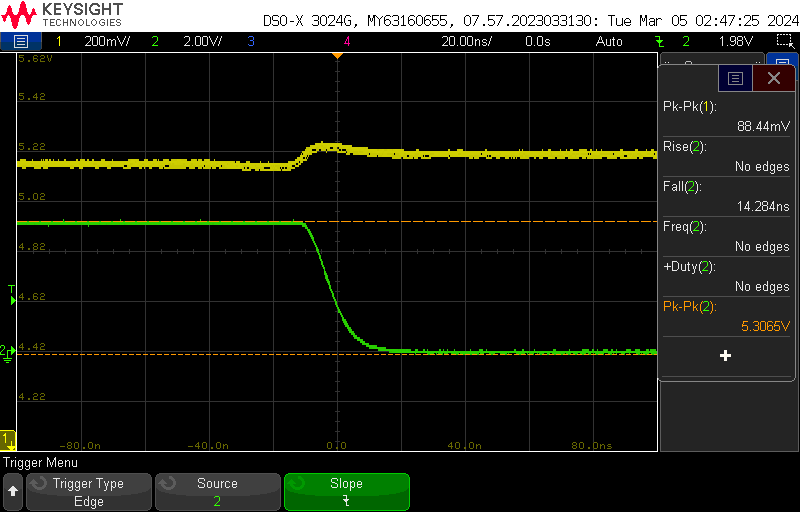
\includegraphics[scale=0.6]{figures/good/quite_high/fall/falling_qh_good6.png}
			\caption{Good layout Quite High Rise \& Fall time with load connected}
		\end{figure}
		\item Results:\\
		Noise at 80.40 mV with a rise time of 15 ns.\\
		Noise at 88 mV with a fall time of 14.28 ns.
	\end{itemize}
	
	\item Noise at Quiet Low (Rise/Fall):
	\begin{itemize}
		\item Objective: Measure and compare the switching noise at quiet low with the bad layout.
		\item 
		\begin{figure}[H]
			\centering
			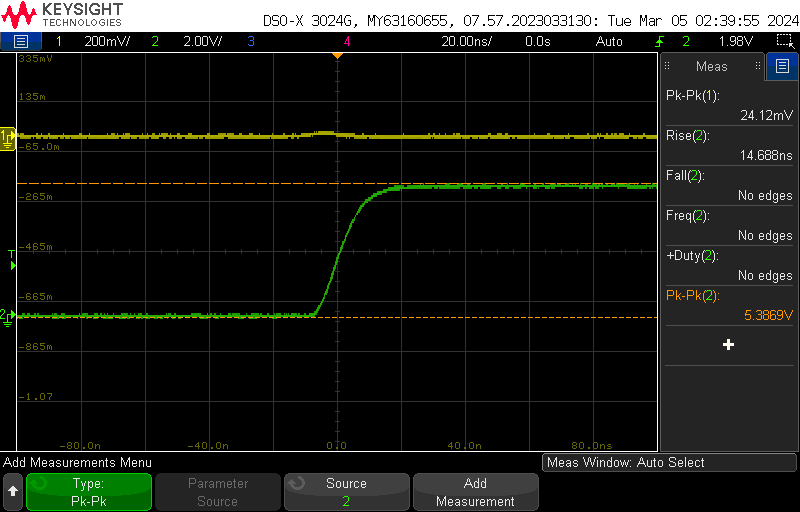
\includegraphics[scale=0.6]{figures/good/quite_low/rise/rising_good_low.png}
			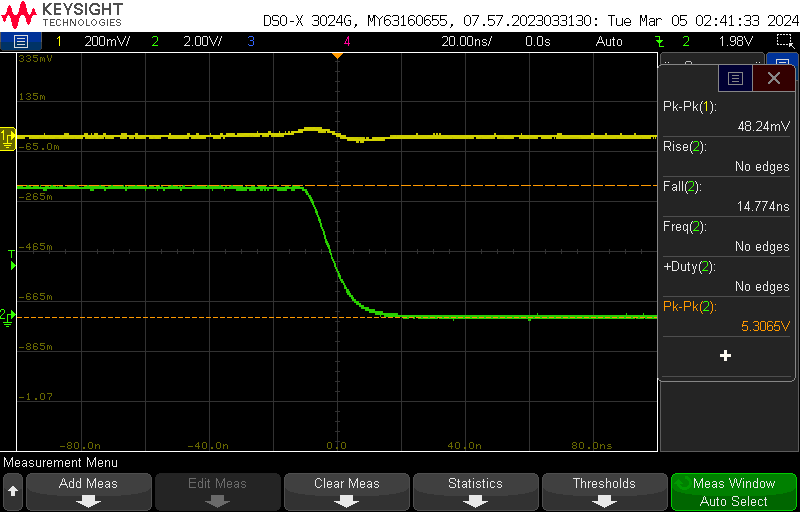
\includegraphics[scale=0.6]{figures/good/quite_low/fall/falling_ql_good.png}
			\caption{Good layout Quite Low Rise \& Fall time with load connected}
		\end{figure}
		\item Results:\\
		Noise at 24 mV with a rise time of 14.688 ns.\\
		Noise at 48.24 mV with a fall time of 14.774 ns.\\
	\end{itemize}
	
\end{enumerate}

\subsection{\textbf{Overview:}}

\begin{table}[H]
	\centering 
	\begin{tabular}{ |l |c | c|}
		\hline
		\textbf{Layout}&\textbf{Quite High Noise}&\textbf{Quite Low Noise}\\\hline
		&&\\
Good Layout& 
\begin{tabular}{@{}cc@{}} % Inner table with two columns
	\textbf{Rise} & \textbf{Fall} \\
	80.4 mV & 88 mV \\
\end{tabular} &
\begin{tabular}{@{}cc@{}} % Inner table with two columns
	\textbf{Rise} & \textbf{Fall} \\
	24 mV & 48 mV \\
\end{tabular}\\

Bad Layout&
\begin{tabular}{@{}cc@{}} % Inner table with two columns
	418.09 mV & 466.33 mV \\
\end{tabular} &
\begin{tabular}{@{}cc@{}} % Inner table with two columns
	64.32mV & 72.36mV \\
\end{tabular} \\

\hline\hline
	\end{tabular}
	\caption{Noise Measurement}
	\label{filterspecs}
\end{table}



\begin{table}[H]
	\centering 
	\begin{tabular}{l c  c}
		\hline
		\textbf{Layout}&\textbf{Rise Time}&\textbf{Fall Time}\\\hline
		&&\\

Good Layout&14.688 ns&14.7 ns\\
Bad Layout&15.469 ns&14.47 ns$\mu$F\\
\hline\hline
	\end{tabular}
	\caption{Rise Time / Fall time}
	\label{filterspecs}
\end{table}

\section{Calculating Thevenin resistance for Hex board}


		Without Load Resistance: The open-circuit voltage Voc
  is measured across the terminals, which is equivalent to the Thevenin voltage Vth\\

		With Load Resistance: The circuit voltage Vload
  is measured again after reintroducing the load resistance of 50$\ohm$.\\

	\begin{flalign*}
	\label{equation_th}
	R_{th} = R_{load}\left(\frac{V_{th} - V_{load}}{V_{load}} \right)
	\end{flalign*}

	\pagebreak

	So first we will measure voltage without load resistance

	We got around 5V of voltage in without load Resistance $R_{load}$.

	Now we will measure Thevenin voltage with load resistance $R_{load}$ of 50$\ohm$.
	
	\begin{figure}[H]
		\centering
		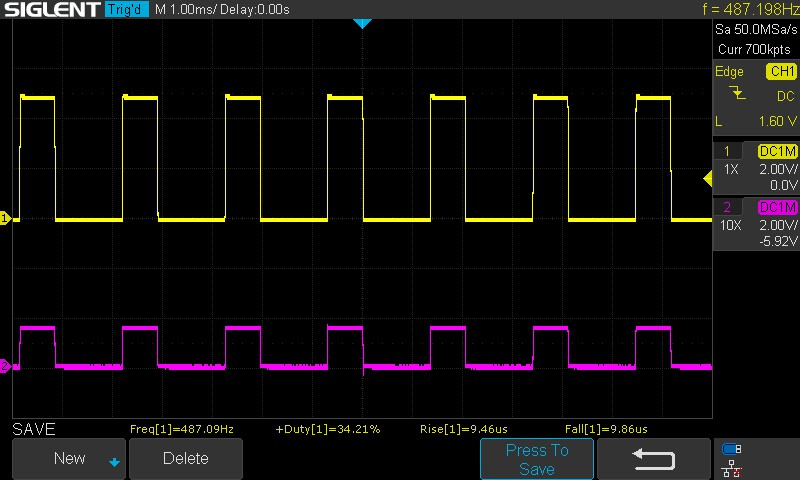
\includegraphics[scale=0.6]{figures/th.jpg}
		\caption{Voltage drop due to load resistance}
	\end{figure}

	This time, We got around voltage drop of \textbf{1.6V} across the load resistance of 50$\ohm$.

	and putting values in the equation \ref{equation_th} will give us,

	\begin{flalign*}
		&R_{th} = 50 \left(\frac{5 - 3.6}{3.6} \right)&&\\
		&R_{th} = 50 \cdot 0.38&&\\
		&\boxed{R_{th} = 19\ohm}\\
	\end{flalign*}
	

	So conclusion is that the $R_{th}$ of power supply would be around 19$\ohm$.

	\section{Current through the LED’s}
	\begin{flalign*}
		&I_{r} = voltage across resistor \cdot Load Resistor &&\\
		&I_{r} = 1.6 \cdot 50 &&\\
		&\boxed{I_{r} = 0.032 A}\\
	\end{flalign*}

\section{What worked ?}

\begin{table}[H]
	\centering

	\begin{tabular}{l c}

		\textbf{Parameter}&\textbf{Worked ?}\\\hline
		5V Input&\ding{51}\\
		Desired frequency of Output&\ding{51}\\
		Duty cycle as calculated&\ding{51}\\
		Low switching noise for good layout&\ding{51}\\
		High switching noise for bad layout&\ding{51}\\
		Current across LEDs&\ding{51}\\

	\end{tabular}
	\caption{Rise-time and Fall-time}
	\label{tab_rise_fall}
\end{table}

\section{Mistakes Made}

\textbf{Overview of Mistakes and Adjustments}
Everything was working as expected, i could have used smaller board size in PCB

\section{Learnings}

The lab demonstrated the characteristics of 555 timer ICs in various configurations(555 timer circuit set up as an astable multivibrator). The primary objectives were met. And creating 2 layer PCB with understanding of how to use altium, debug the PCB and use theoretical knowledge to create it in software and implement in PCB.\\

Here are the key lessons learned:\\
\begin{enumerate}
	\item Decoupling Capacitors' Impact: The placement of decoupling capacitors is critical. Their effectiveness in reducing power rail switching noise is inversely proportional to their distance from the IC; the closer they are, the less noise.
	\item Cross Talk Phenomena: In the absence of a continuous ground return path, especially in the poorly designed layout, two distinct types of cross talk were identified:
	\begin{itemize}
		\item 
		The first type is linked to the power path and particularly influences the 'Quite High' pin.
		\item The second type is inductive cross talk, attributed to the lack of a continuous ground plane, impacting the 'Quite Low' pin.
	\end{itemize}
	\item Significance of Ground Return Path: The absence of a ground return path in the bad layout created an environment conducive to cross talk, which affects signal integrity.
	\item 
	Noise Comparison Between Layouts: A marked difference in switching noise was observed when comparing the 'Quite Low' and 'High' pins across the bad and good layout sides, with the bad layout exhibiting more noise.
	\item Effective Noise Reduction: Adherence to best layout practices, such as maintaining a continuous ground plane and placing decoupling capacitors close to their associated ICs, can significantly mitigate switching noise.
\end{enumerate}











\vfill
\hrule
\vspace{0.5cm}



\vspace{1cm}
\hrule
\vspace{0.5cm}


%---------------------------------------------------------------------------
\end{document}
-
